 
%\part{Variables aleatorias}
%\frame{\titlepage}

\chapter{Variables aleatorias. Distribuciones notables}
%\frame{\tableofcontents}


%\part{Variables aleatorias. Distribuciones notables}

\section{Variables aleatorias}

\begin{frame}

\frametitle{Variables Aleatorias}

\begin{itemize}
\item Consideremos un experimento aleatorio y con espacio muestral $\Omega$. 
\item Una \textbf{variable aleatoria} (v.a) es una  aplicación (que cumple algunas propiedades adicionales)
$$X:\Omega\to \RR.$$ 
\item Es decir es una aplicación que transforma sucesos elementales del especio muestral en  un número real.
\end{itemize}

\end{frame}

\begin{frame}
    \frametitle{Variables aleatorias discretas y continuas}
\begin{itemize}
\item Llamaremos \textbf{dominio} de una variable aleatoria $X$ al conjunto $D_X=X(\Omega)$. Es decir el dominio de una v.a. es el cojunto de valores reales que asume.
\item 
    Diremos que una v.a. $X$ es \textbf{discreta}, o más exactamente que tiene dominio discreto, si el conjunto $D_X$ es
    finito o numerable. Lo denotaremos por 
    $D_X=\{x_{1},\ldots,x_{n},\ldots \}$
    (normalmente $x_{1}<x_{2}<\ldots<x_{n}\ldots$) si es infinito y por 
  
    $D_X=\{x_{1},\ldots,x_{n}\}$ si es finito.
\item Diremos que una variable es continua, o más exactamente que tiene dominio continuo,  si $D_X$ es uno o varios intervalos  de la recta real. 
\end{itemize}              
\end{frame}


% \begin{frame}
%     \begin{itemize}
%     \item Sea $X:\Omega \to \RR$ una aplicaci\'on tal que
%     $X(\Omega)=\{x_{1},\ldots,x_{n},\ldots\}$ entonces
% 
%     $X$ es v.a. discreta sii $X^{-1}(\{x_{k}\})=\{\omega\in\Omega |
%     X(\omega)=x_{k}\}\in\mathcal{F}$ para todo $x_{k}\in X(\Omega)$
% 
%     Normalmente pondremos \newline $X^{-1}(x_{k})=\{X=x_{k}\}$
%     \item Si $\Omega$ es finito toda v.a. $X:\Omega\to \RR$ es discreta
%     sobre $(\Omega, \mathcal{F},P)$
%     \item Si $X$ e $Y$ son dos v.a. discretas entonces $X+Y$ y $X\cdot Y$ son
%     tambi\'en v.a. discretas.
%     \item Si $X$ es una v.a. discreta y $h:\RR\to\RR$ una aplicaci\'on
%     entonces $h(X):\Omega\to \RR$  definida por
%     $(h(X))(\omega)=h(X(\omega))$ es tambi\'en una v.a. discreta.
%     \end{itemize}
%               \end{frame}

\subsection{Funciones de distribución}
\begin{frame}
\frametitle{Sucesos con variables aleatorias}

Una vez tenemos una variable aleatoria podemos definir diferentes sucesos, estos suelen tener una  notación peculiar. Veamos unos ejemplos:

\begin{itemize}
\item El suceso $\{X=x\}$, habitualmente se representa sin llaves: $P(X=x)$.
\item El suceso $\{X\leq x\}=\{X \in (-\infty,x]\}$ habitualmente se representa sin llaves: $P(X\leq x)$.
\item El suceso $\{a< X\leq b\}=\{X \in (a,b]\}$ habitualmente se representa sin llaves: $P(a< X \leq b)$.
\item Y otros sucesos que se definen de forma similar.
\item Para la operación unión de sucesos utilizaremos el símbolo convencional $\cup$. Por ejemplo el suceso que $X>3$ o $X<-1$ lo  escribiremos como $P(\{X>3\} \cup \{X<-1\})$.
\item En cambio para la intersección se suelen poner comas: $P(1<X, X\leq 3)$  es $P(\{1<X\}\cap \{X\leq 3\})$.   
\end{itemize}
\end{frame}




\begin{frame}
\frametitle{Funci\'on de distribuci\'on}
\begin{itemize}
 \item  \textbf{Llamaremos funci\'on de distribuci\'on (acumulada)} o \textbf{funci\'on de probabilidad acumulada} de una v.a. $X$
a la funci\'on $F:\RR\to [0,1]$ definida por
       $$F(x)=P(X\in (-\infty,x])=P(X\leq x)$$
\end{itemize}
\end{frame}

\begin{frame}
\frametitle{Propiedades}
\begin{itemize}
\item      Sea $F$ una funci\'on de  distribución acumlada de la v.a. $X$ entonces:
\begin{enumerate}[a)]
 \item $F$ es creciente.
 \item $F$ es continua por la derecha.
\item  $\displaystyle\mbox{lím}_{x\to\infty}F(x)=1$;
           $\mbox{lím}_{x\to-\infty}F(x)=0$.
\item $0\leq F(x)\leq 1$.
\item  Toda funci\'on $F$ verificando a), b) y c) es funci\'on de
           distribuci\'on de alguna v.a. $X$.
\end{enumerate}
\end{itemize}

\end{frame}

\begin{frame}
\frametitle{Propiedad}
Sea $F$ una funci\'on de distribuci\'on de la v.a. $X$ entonces dados $a,b\in\RR$ con $a<b$
\begin{itemize}
\item $P(X\geq a)=1-P(X\leq a)=1-F(a)$.
\item $P(X<a)=P(X\leq a)-P(X=a)=F(a)-P(X=a)$.
\item $P(a<X\leq b)=P(X\leq b)-P(X\leq a)=F(b)-F(a)$.
\end{itemize}
\end{frame}

\begin{frame}
\frametitle{Más propiedades}

Si denotamos por $F(x_{0}^{-})=\mbox{lím}_{x\to x_{0}^{-}} F(x)$.
        
\begin{enumerate}[a)]
\item $P(X=x)=P(X\leq x)-P(X<x)=F(x)-F(x^{-})$.
\item $P(X<a)=F(a^{-})$.
\item $P(X\geq a)=1-P(X<a)=1-F(a^{-})$.
\item $P(X> a)=1-F(a)$.
\item $P(a\leq X\leq b)=F(b)-F(a^{-})$.
\item $P(a< X< b)=P(X<b)-P(X\leq a)=F(b^{-})-F(a)$.
\item $P(a\leq X< b)=P(X<b)-P(X< a)=F(b^{-})-F(a^{-})$.
\end{enumerate}
\end{frame}

\subsection{Cuantiles}
\begin{frame}
\frametitle{Cuantiles de una distribución}
\begin{itemize}
\item Llamaremos \textbf{cuantil} de orden $p$ de la v.a. $X$ al valor $x_p$, si existe, tal que $P(X\leq x_p)=F(x_p)=p$.
\item En caso de que no exista ese valor, suele pasar con varibles discretas, se toma como \textbf{cuantil} el valor más pequeño tal que $P(X\leq x_p)=F(x_p)\geq p$.
\item Los cuantiles de las distribuciones son las versiones poblacionales de los cuantiles muestrales.
\item En este tema, y en los que siguen, a medida que sea necesario iremos exponiendo el cálculo de los cuantiles de las distribuciones de probabilidad que necesitemos.
\end{itemize}
\end{frame}
\section{Variables aleatorias discretas}
\subsection{Función probabilidad variables discretas}
\begin{frame}

    \frametitle{Función de probabilidad de una v.a. discreta}

    Sea $X$ una v.a. discreta con
    $D_X=\{x_{1},x_{2},\ldots,x_{n},\ldots\}$. Llamaremos ley
    de probabilidad, funci\'on de probabilidad o función de cuantía de la v.a. $X$ a la
    funci\'on $f:\RR\to\RR$ definida por 
$$f(x)=P(X=x),$$ 

para todo
    $x\in\RR$.
% 
%     Notar que $f_{X}(x)=P(X=x)=P(X^{-1}(x))$ y por lo tanto
%     si $x\not\in X(\Omega)$ entonces
%     $f_{X}(x)=P(X=x)=P(X^{-1}(x))=P(\emptyset)=0$
\end{frame}



\begin{frame}
     \textbf{Propiedad}
     Sea $X$ una v.a. discreta con funci\'on de probabilidad $f$
     entonces:
     \begin{enumerate}[a)]
         \item $\displaystyle \sum_{x\in D_X} f(x)=1$; $f(x)=0$ si
         $x\not\in D_X$.
         \item $$P(X\leq a)=\sum_{\begin{array}{c}x\in
         X(\Omega)\\ x\leq a\end{array}} f(x)$$

         \end{enumerate}
          \end{frame}

\subsection{Valor esperado y varianza para variables discretas}
\begin{frame} 
\frametitle{Esperanza y varianza para variables aleatorias discretas}
Sea $X$ una v.a. discreta con función de probabilidad $f$ y dominio $D_X$
\begin{itemize} 
\item Se define el valor esperado, esperanza o media como 
$E(X)=\sum_{x\in D_X} x\cdot f(x)$.
\item Si $H:\RR\to \RR$ es una función se define:
$E(H(X))=\sum_{x\in D_X} H(x)\cdot f(x)$.
\item Se define la varianza por $Var(X)=E((X-E(X))^2)=E(X^2)-E(X)^2$.
\item La desviación típica es $\sqrt{Var(X)}$.
\item Habitualmente se utilizan las letras griegas $\mu$, $\sigma^2$  y $\sigma$ para representar la esperanza,  la varianza y la desviación típica.
\end{itemize}
\end{frame}

\begin{frame}
\frametitle{Propiedades}
\begin{enumerate}[a)]
\item $E(cte.)=cte$
 \item $E(a X+b)=a E(X)+b$
% \item $\displaystyle  E\left(\sum_{k=1}^{n }g_{k}(X)\right)=
%                 \sum_{k=1}^{n }E\left(g_{k}(X)\right)$
\item Si $a<X<b$ entonces $a<E(X)<b$
\item Si $X$ es una v.a. no negativa entonces $E(X)\geq 0$.
\item Si $g(X)\leq h(X)$ entonces $E(g(X))\leq E(h(X))$
\item $Var(a X+b)=a^2 Var(x)$.
\end{enumerate}
\end{frame}


%ppppppppppp
\begin{frame}
\frametitle{Ejemplo}
La tabla siguiente muestra la función de probabilidad asociada a la variable aleatòria $X$ ``número de batidos de ala por segundo en individuos de una especie de mariposa''
\begin{center}
\begin{tabular}{l|ccccc}
$x$ & 6 & 7 & 8 & 9 & 10\\
\hline
$f(x)$ &  0.05 & 0.1 & 0.6 & 0.15 & ?
\end{tabular}
\end{center}

¿Cuál es el valor de la entrada que  falta?
$$
\begin{array}{rl}
1 & =f(6)+f(7)+f(8)+f(9)+f(10)\\ & =0.05+0.1+0.6+0.15+f(10)\\ & = 0.9+f(10)\Rightarrow f(10)=0.1
\end{array}
$$
\end{frame}

\begin{frame}
\frametitle{Ejemplo}
\begin{center}
\begin{tabular}{l|ccccc}
$x$ & 6 & 7 & 8 & 9 & 10\\
\hline
$f(x)$ &  0.05 & 0.1 & 0.6 & 0.15 &  0.1
\end{tabular}
\end{center}
¿Cual es la función de distribución acumulativa?
\medskip

Se producen saltos en  $6, 7, 8, 9, 10$:
$$
F(x)=\left\{
\begin{array}{ll}
0 & \mbox{ si $x<6$}\\
0.05 & \mbox{ si $6\leq x< 7$}\\
0.15 & \mbox{ si $7\leq x< 8$}\\
0.75 & \mbox{ si $8\leq x< 9$}\\
0.9 & \mbox{ si $9\leq x< 10$}\\
1 & \mbox{ si $10\leq x$}
\end{array}\right.
$$


\end{frame}

\begin{frame}
\frametitle{Ejemplo}
\begin{center}
\begin{tabular}{l|ccccc}
$x$ & 6 & 7 & 8 & 9 & 10\\
\hline
$f(x)$ &  0.05 & 0.1 & 0.6 & 0.15 &  0.1
\end{tabular}
\end{center}
¿Cual es la distribución acumulada?
\vspace*{-5ex}
\begin{center}
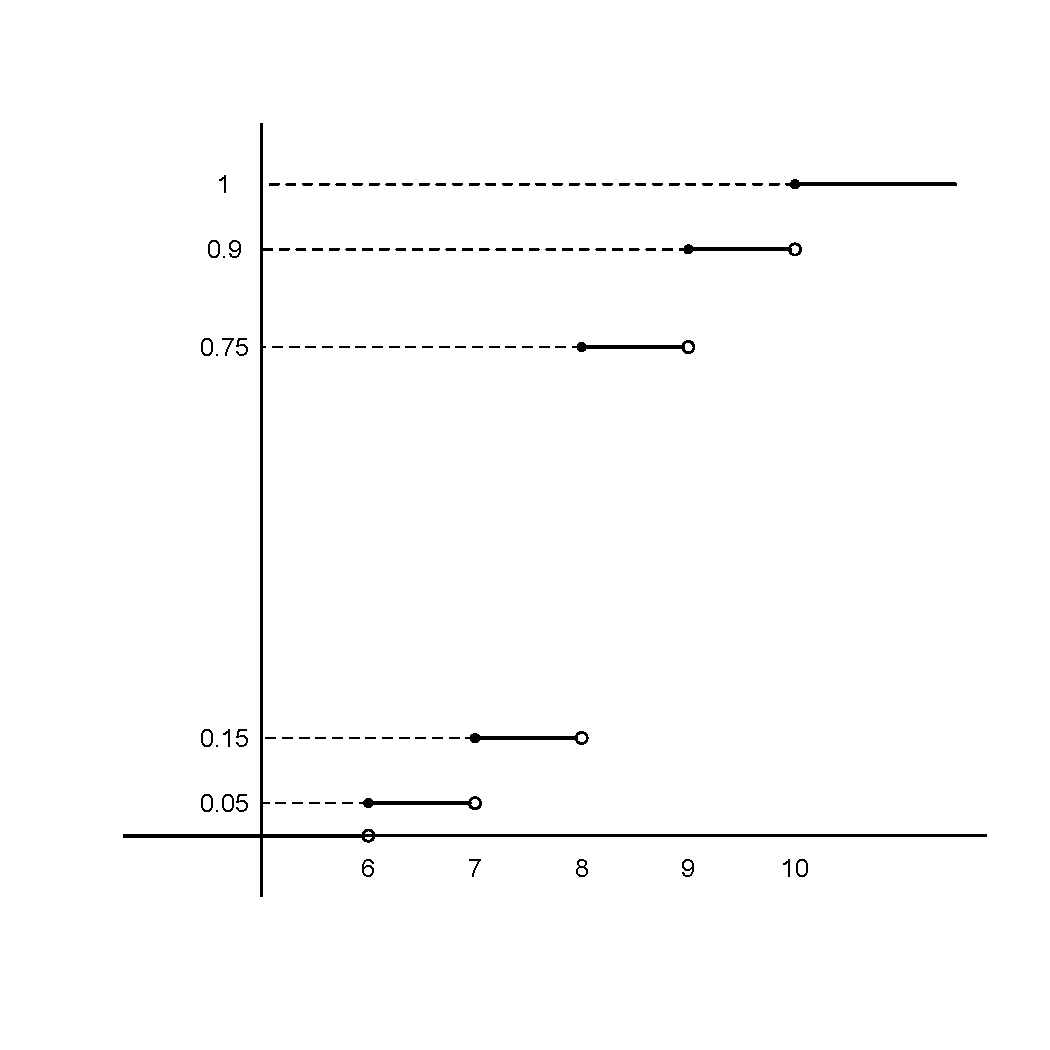
\includegraphics[height=6cm]{distr1.pdf}
\end{center}

\end{frame}


\begin{frame}
\frametitle{Ejemplo}
Si nos dan la distribución $F:S\to [0,1]$, con 
$$
D_X=\{6,7,8,9,10\},
$$
 ¿cómo calcularias la función de probabilidad?
\vspace*{-5ex}

\begin{center}
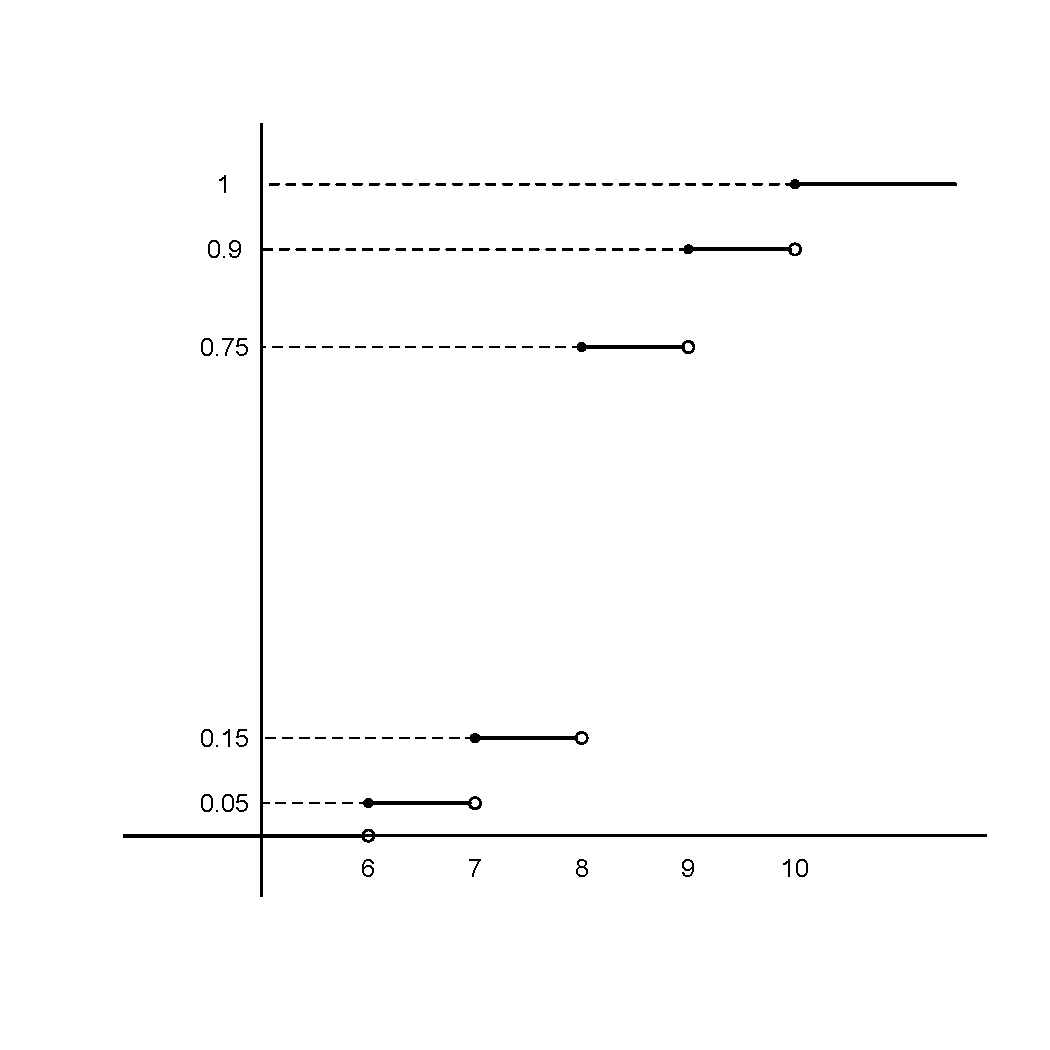
\includegraphics[height=6cm]{distr1.pdf}
\end{center}

\end{frame}


\begin{frame}
\frametitle{Ejemplo}
$D_X=\{6,7,8,9,10\}$
\medskip

$f(6)=0.05,\ f(7)=0.15-0.05=0.1$

$f(8)=0.75-0.15=0.6,$

$f(9)=0.9-0.75=0.15, f(10)=1-0.9=0.1$
\vspace*{-5ex}

\begin{center}
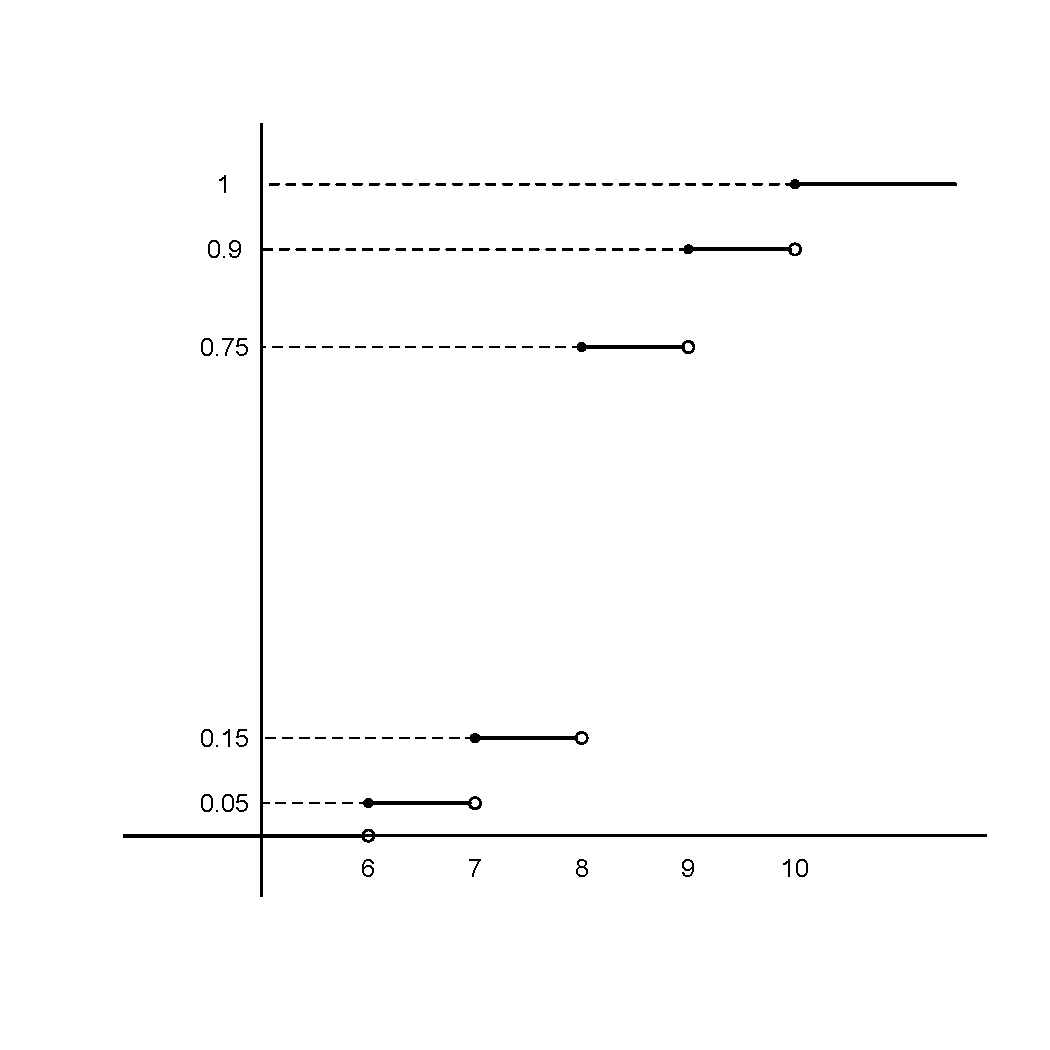
\includegraphics[height=6cm]{distr1.pdf}
\end{center}

\end{frame}


\begin{frame}
\frametitle{Ejemplo}
La tabla siguiente nos da la función de probabilidad asociada a la variable aleatoria $X$ ``número de batidos de ala por segundo en individuos de una determinada especie de mariposas''
\begin{center}
\begin{tabular}{l|ccccc}
$x$ & 6 & 7 & 8 & 9 & 10\\
\hline
$f(x)$ &  0.05 & 0.1 & 0.6 & 0.15 & 0.1
\end{tabular}
\end{center}

¿Cuál es el valor esperado del número de batidas?
\medskip

$$
E(X)=6\cdot f(6)+7\cdot f(7)+8\cdot f(8)+9\cdot f(9)+10\cdot f(10)=8.15
$$
\end{frame}

\begin{frame}
\frametitle{Ejemplo}
La tabla siguiente nos da la función de probabilidad asociada a la variable aleatoria $X$ ``número de batidos de ala por segundo en individuos de una determinada especie de mariposas''
\begin{center}
\begin{tabular}{l|ccccc}
$x$ & 6 & 7 & 8 & 9 & 10\\
\hline
$f(x)$ &  0.05 & 0.1 & 0.6 & 0.15 & 0.1
\end{tabular}
\end{center}

¿Cuál es el  valor esperado de $X^2$?
$$
\begin{array}{rl}
E(X^2)  & = 6^2\cdot f(6)+7^2\cdot f(7)+8^2\cdot f(8) +9^2\cdot f(9)\\ & \quad+10^2\cdot f(10) =67.25
\end{array}
$$
\textbf{¡Alerta!} $E(X^2)\neq E(X)^2$ ($67.25\neq 8.15^2=66.4225$)
\end{frame}

\begin{frame}
\frametitle{Ejemplo}
La tabla siguiente nos da la función de probabilidad asociada a la variable aleatoria $X$ ``número de batidos de ala por segundo en individuos de una determinada especie de mariposas''
\begin{center}
\begin{tabular}{l|ccccc}
$x$ & 6 & 7 & 8 & 9 & 10\\
\hline
$f(x)$ &  0.05 & 0.1 & 0.6 & 0.15 & 0.1
\end{tabular}
\end{center}

¿Cuánto valen la varianza y la desviación típica de $X$? ($E(X)=8.15$)
{\small $$
\begin{array}{rl}
Var(X) \!\!&\!\! =(6-8.15)^2\cdot f(6)+(7-8.15)^2\cdot f(7)\\ & \quad +(8-8.15)^2\cdot f(8)+(9-8.15)^2\cdot f(9)\\ & \quad +(10-8.15)^2\cdot f(10)=0.8275\\
Var(X)  \!\!&\!\! =E(X^2)-E(X)^2=67.25-8.15^2=0.8275\\
\sigma(X)  \!\!&\!\! =\sqrt{Var(X)}=\sqrt{0.8275}\approx 0.90967
\end{array}$$
}
\end{frame}



%\subsection{Distribuciones discretas notables}
%%ppppppppppp
\section{Algunas distribuciones de probabilidad discretas}
\subsection{Distribución  Bernouilli}
\begin{frame}
    \frametitle{Distribución Bernoulli}
    Consideremos un experimento con dos resultados posibles \'exito (E) y
    fracaso (F). Sea $\Omega=\{E,F\}$ el espacio muestral asociado al experimento.
    De forma que sabemos que  $P(E)=p$ y $P(F)=1-p=q$ con $0<p<1$.
    Consideremos la  aplicaci\'on $X:\Omega=\{E,F\}\to \RR$ definida por
    $X(E)=1$, $X(F)=0$ entonces su  funci\'on de probabilidad es
    $$f(x)=\left\{\begin{array}{ll} q & \mbox{si } x=0\\
    p & \mbox{si } x=1\\
    0 & \mbox{en cualquier otro caso}\end{array}\right.$$

    Bajo estas condiciones diremos que $X$ sigue una distribuci\'on de probabilidad  \textbf{Bernoulli} de par\'ametro $p$ y lo denotaremos por  $Ber(p)$ o $B(1,p)$. A los experimentos de este tipo \newline(\'exito/fracaso) se les denomina experimentos Bernoulli.
\end{frame}
\subsection{Distribución  Binomial}
\begin{frame}
\frametitle{Distribución Binomial}
 Supongamos que repetimos $n$ veces de forma
    independiente un experimento Bernoulli de par\'ame\-tro $p$. Entonces
    $\Omega$ estar\'a formado por cadenas de $E$'s y $F$'s de longitud $n$.

    Sea $X:\Omega\to\RR$ definida por $X(\omega)=$n\'umero de \'exitos en
    $\omega$. Entonces $f(k)=P(X=k)=\left(\begin{array}{cc} n\\
    k\end{array}\right)
    p^k (1-p)^{n-k}$ si $k=0,1,\ldots,n$  siendo nula en el resto de casos.

    Entonces diremos que la v.a. sigue una \textbf{ley de probabilidad binomial}
    con par\'ametros $n$ y $p$ y lo denotaremos por $B(n,p)$. (Nota:
    $B(1,p)=Ber(p)$)
\end{frame}


\begin{frame}
\frametitle{Resumen Binomial}
Sea $X$ una v.a. con distribución $B(n,p)$.
\begin{center}
\scalebox{0.80}[0.8]{ 
\begin{tabular}{|c|c|c|c|c|}
\hline \begin{tabular}{c} Valores\\ admisibles.\end{tabular} & $P_X(x)=P(X=x)=$ &
$\begin{array}{l}F(x)=\\P(X\leq X)=\end{array}$ &
 $E(X)$ & $Var(X)$\\\hline & & & &\\
 $D_X=\{0,1,\ldots,n\}$ &
 $\left\{
 \begin{array}{ll}
{n\choose x} p^x q^{n-x} & \mbox{ si } x=0,1,\ldots,n\\
     0  & \mbox{ en otro caso
}\end{array}\right.$  & Tabulada & $n p$ & $n p q$ \\& & & &\\ \hline
\end{tabular} }
\end{center}
\end{frame}


%%%%pppp

\begin{frame}
\frametitle{\texttt{R} y las distribuciones de probabilidad}
\texttt{R} conoce las distribuciones de probabilidad más importantes, por ejemplo la binomial (\texttt{binom}).
\medskip

Dada una distribución
\begin{itemize}
\item Añadiendo el prefijo \texttt{d}, obtenemos la correspondiente función de probabilidad ( o de densidad): por ej., de la binomial, \texttt{dbinom}

\item Añadiendo el prefijo \texttt{p}, obtenemos la correspondiente distribución acumulativa: por ej.., de la binomial, \texttt{pbinom}

\item Añadiendo el prefijo \texttt{q}, obtenemos el cuantil de  la correspondiente distribución acumulativa: por ej.., de la binomial, \texttt{qbinom}
\item Añadiendo el prefijo \texttt{r}, obtenemos muestras aleatorias de esa distribución: por ej.., de la binomial, \texttt{rbinom}
\end{itemize}
\end{frame}

\begin{frame}[fragile]
\frametitle{Con  \texttt{R}}
Por ejemplo, si estamos usando una  $B(20,0.3)$

\begin{Schunk}
\begin{Sinput}
> dbinom(5, 20, 0.3)
\end{Sinput}
\begin{Soutput}
[1] 0.1788631
\end{Soutput}
\begin{Sinput}
> pbinom(5, 20, 0.3)
\end{Sinput}
\begin{Soutput}
[1] 0.4163708
\end{Soutput}
\begin{Sinput}
> qbinom(0.5, 10, 0.3)
\end{Sinput}
\begin{Soutput}
[1] 3
\end{Soutput}
\begin{Sinput}
> rbinom(10, 5, 0.3)
\end{Sinput}
\begin{Soutput}
 [1] 2 0 1 3 1 2 2 1 1 3
\end{Soutput}
\end{Schunk}



Nos dan respectivamente:
\end{frame}


\begin{frame}

\begin{itemize}
\item \texttt{dbinom(5,20,0.3)} nos da el valor de la función densidad en el 5, $f(5)$.
\item \texttt{pbinom(5,20,0.3)} nos da el valor de la distribución acumulada en  5,  $F(5)$.
\item \texttt{qbinom(0.5,10,0.3)} nos da el $Q_{0.5}$  la mediana para la distribución acumulada.
\item \texttt{rbinom(10,5,0.3)} nos da diez números aleatorios de una $B(5,0.3)$. 
\end{itemize}

% \begin{verbatim}
% > dbinom(5,20,0.3)
% [1] 0.1788631
% > pbinom(5,20,0.3)
% [1] 0.4163708
% > pbinom(20,20,0.3)
% [1] 1
% \end{verbatim}
\end{frame}


\begin{frame}
\frametitle{Ejemplo}
%$f(k)=\binom{n}{k}p^k(1-p)^{n-k}$
% \red{$f(k)=\binom{n}{k}p^k(1-p)^{n-k}$}
% \medskip
En una cierta enfermedad, la probabilidad que un hijo de madre enferma enferme es  $0.5006$. Una mujer enferma tiene $4$ hijos.
\medskip

¿Cuál es la probabilidad de que tenga exactamente un hijo enfermo?
\medskip

$X=$ número de hijos enfermos de la  madre enferma.
\medskip
una distribución  $B(4,0.5006)$. Por  lo tanto
$$
P(X=1)=f(1)=\binom{4}{1}0.5006^1\cdot 0.4994^3=\ldots
$$

\end{frame}


\begin{frame}
\frametitle{Ejemplo}
$f(k)=\binom{n}{k}p^k(1-p)^{n-k}$
\medskip

 En una cierta enfermedad, la probabilidad que un hijo de madre enferma enferme es  $0.5006$. Una mujer enferma tiene $4$ hijos.
\medskip

¿Cuál es la probabilidad de que tenga al menos un hijo enfermo?
\medskip\pause

$X=$ número de hijos enfermos de la  madre enferma.
\medskip


Que sigue una ley de distribución $B(4,0.5006)$. Por lo tanto
{\small $$
\begin{array}{l}
P(X\geq 1)= P(X=1)+P(X=2)+P(X=3)+P(X=4)\\
\quad =f(1)+f(2)+f(3)+f(4)\\
\quad =\binom{4}{1}0.5006^1\cdot 0.4994^3+\binom{4}{2}0.5006^2\cdot 0.4994^2\\ \qquad +\binom{4}{3}0.5006^3\cdot 0.4994^1+\binom{4}{4}0.5006^4\cdot 0.4994^0=\ldots
\end{array}
$$}
\end{frame}


\begin{frame}
\frametitle{Ejemplo}
$f(k)=\binom{n}{k}p^k(1-p)^{n-k}$
%\red{$f(k)=\binom{n}{k}p^k(1-p)^{n-k}$}
\medskip

$X=$ número de hijos enfermos de la  madre enferma.
\medskip

¿Cuál es la probabilidad de que tenga al menos un hijo enfermo?
\medskip\pause

$X=$ número de hijos enfermos de la  madre enferma.
\medskip

Su distribución de probabilidad es  $B(4,0.5006)$. En  esta ocasión la calcularemos de otra manera 
$$
\begin{array}{rl}
P(X\geq 1) & =1-P(X=0)=1-f(0)\\ & =1-
\dbinom{4}{0}0.5006^0\cdot 0.4994^4=\ldots
\end{array}
$$
\end{frame}


\begin{frame}
\frametitle{Ejemplo}
$f(k)=\binom{n}{k}p^k(1-p)^{n-k}$
%\red{$f(k)=\binom{n}{k}p^k(1-p)^{n-k}$}
\medskip

$X=$ número de hijos enfermos de la  madre enferma.
\medskip

¿Cuál es la media y al variaza del número de hijos enfermos?
\medskip\pause


Su distribución de probabilidad es  $B(4,0.5006)$. Por lo tanto $n=4$ y $p=0.5006$. Por lo tanto la esperanza es
$$E(X)= n p = 4\cdot 0.5006,$$

la varianza es,

$$Var(X)= n p q =  4\cdot 0.5006\cdot (1-0.5006).$$

y la desviación típica es $\sqrt{4\cdot 0.5006\cdot (1-0.5006)}$.
\end{frame}

\begin{frame}
\frametitle{Uso de tablas  para el cáculo de la distribución binomial}
\begin{itemize}
\item Tradicionalmente, hace no muchos años, para el cálculo de las probabilidades de la distribución binomial se utilizaban  tablas.
\item Algunas de estas tabla las podéis encontrar en la carpeta de material adicional en el sitio de la asignatura en campus extens.
\item Estas tablas han sido elaboradas con \texttt{R}.
\item Como ejercicio repetir los cálculos anteriores con estas tablas. 
\item \textbf{Atención:} Son estas tablas las que utilizaréis en los controles escritos.
\end{itemize}
\end{frame}

\subsection{Distribución  Geométrica}

\begin{frame}
 \frametitle{Distribución Geométrica} 
\begin{itemize}
\item Consideremos una experiencia consistente en repetir un experimento Bernouilli, de parámetro $p$, de forma independiente hasta obtener el primer éxito.
\item Sea $X$ la v.a. que cuenta el número de fracasos necesarios para obtener el primer \'exito. 
\item Entonces $f(x)=P(X=x)= p(1-p)^{x}$ si $x=0,1,2,\ldots$ siendo nula en el
    resto de casos.
\item  Una v.a. de este tipo diremos que sigue una
    distribuci\'on geom\'etrica de par\'ametro $p$ y lo denotaremos por $Ge(p)$.
\end{itemize}
\end{frame}

\begin{frame}
\frametitle{Resumen Geométrica}
Sea $X$ una v.a. $Ge(p)$.

\scalebox{0.7}[0.7]{ 
\begin{tabular}{|c|c|c|c|c|}
 \hline
\multicolumn{5}{|c|}{$X=$ número de fracasos  para conseguir el primer éxito.}\\
 \hline \begin{tabular}{c} Valores\\ admisibles.\end{tabular} &
$P_X(x)=P(X=x)=$ & $F(x)=P(X\leq x)=$&
 $E(X)$ & $Var(X)$\\\hline & & & &\\
  $\begin{array}{l}D_X=\\\{0,1,\ldots\}\end{array}$  & $\left\{\begin{array}{ll}
 q^k p & \mbox{ si } k=0,1,2,\ldots\\
 0 &\mbox{ en otro caso}
    \end{array}\right.$  &
$\left\{\begin{array}{ll} 0 & \mbox{si } x<0\\
 1- q^{k+1} & \mbox{si }
 \left\{
 \begin{array}{l}
 k\leq x< k+1\\
  \mbox{para } k=0,1,2,\ldots
 \end{array}\right.
    \end{array}\right.$  & $\frac{q}{p}$ & $\frac{q}{p^2}$ \\& & & &\\ \hline
\end{tabular}
}
\end{frame}


\begin{frame}
    \frametitle{Propiedad de la carencia de memoria}
    Sea $X$ una v.a. discreta, con dominio $D_X=\{0,1,2,3\ldots\}$. Entonces
    $X$ sigue una ley $Ge(p)$ sii $P(X\geq k+j/X> j)=P(X\geq k)$ para
    todo $k,j=1,2,3\ldots$ y $P(X=0)=p$
 \end{frame}

\begin{frame}
\frametitle{Ejemplo}
\begin{itemize}
\item Supongamos que repetimos sucesivamente varias veces cultivos  de unas pruebas analíticas, por ejemplo de orina humana.
\item  En ocasiones el cultivo se puede contaminar y se invalida la prueba. 
\item El motivo de la contaminación puede ser diverso. Se estima que sucede en 1 de cada 10 casos y es fácilmente detectable por la abundacia de tipos de microorganismos presentes de forma natural en el individuo que aparecen en el cultivo. 
\item Consideremos la variable $X$ que nos da el número de análisis consecutivos sin error.
\end{itemize}

Suponiendo independencia entre cada análisis modelizar la variable $X$ mediante una ley geométrica. Calcular $P(X>5), P(X=2), P(X\leq 3)$ y la esperanza, varianza y desviación típica de $X$. Interpretar los resultados.

\end{frame}

\begin{frame}
\frametitle{Ejemplo: el problema de las llaves}
\begin{itemize}
\item Llegamos a casa  de noche  después  después de una fiesta. 
\item Para abrir la puerta de nuestra casa, que sólo tiene una cerradura, disponemos de  5 llaves.
\item Tenemos la mala suerte de que se ha estropeado la luz en la puerta de nuestra casa, de forma que estamos totalmente a oscuras.
\item Nos disponemos a  abrir la puerta eligiendo al azar una llave.
\item  Como estamos ``cansados'' cada vez ``olvidamos'' (no tenemos memoria) la llave utilizada.
\end{itemize}
\end{frame}

\begin{frame}
\frametitle{Ejemplo: el problema de las llaves}
Sea $Y$ la variable que nos da el número de intentos necesarios para abrir la puerta. Notemos que en este caso se  incluye el intento exitoso. Modelizar $Y=X+1$ donde $X$ sea una variable geométrica. Calcular $P(Y>3), P(Y\leq2)$ y $P(X=5)$. Calcular la esperanza, varianza y desviación típica de $Y$.

Responder a la siguiente pregunta ¿si ya he hecho 10 intentos fallidos, cuál es la probabilidad de que tenga que hacer 10 más hasta abrir la  puerta?
\end{frame}


%%%%ppppppppppp


\begin{frame}[fragile]
\frametitle{Cálculo probabilidades de la distribución Geométrica con \texttt{R}}

Con \texttt{R}, es \texttt{geom}, dado $p$
\begin{itemize}
\item $f(k)=\mbox{\texttt{dgeom(}}k,\texttt{p)}$

\item $F(k)=\mbox{\texttt{pgeom(}}k,\texttt{p)}$
\end{itemize}
\begin{Schunk}
\begin{Sinput}
> dgeom(0, 0.4)
\end{Sinput}
\begin{Soutput}
[1] 0.4
\end{Soutput}
\begin{Sinput}
> dgeom(5, 0.4)
\end{Sinput}
\begin{Soutput}
[1] 0.031104
\end{Soutput}
\begin{Sinput}
> pgeom(0, 0.4)
\end{Sinput}
\begin{Soutput}
[1] 0.4
\end{Soutput}
\begin{Sinput}
> pgeom(5, 0.4)
\end{Sinput}
\begin{Soutput}
[1] 0.953344
\end{Soutput}
\begin{Sinput}
> pgeom(30, 0.4)
\end{Sinput}
\begin{Soutput}
[1] 0.9999999
\end{Soutput}
\end{Schunk}
\end{frame}

\begin{frame}
\frametitle{Ejemplo}
%\red{$f(k)=p(1-p)^{k-1}$ si $1\leq k$}
Leemos de forma equiprobable bases de una secuencia genómica en la que cada base aparece con la misma frecuencia, hasta que encontremos una A ¿Cuál es la probabilidad de que paremos antes de  leer 4 bases?
\medskip

$Y$= número de bases que hemos de leer para leer una  A
\medskip

La distribución es $Y=X+1$ donde $X$ es una  $G(0.25)$
\medskip 

$P(Y<4)=P(X+1<4)=P(X< 3)=P(X\leq 2)=F(2)= 1-(1-0.25)^{2+1}=\ldots$
\end{frame}




\begin{frame}
\frametitle{Ejemplo}

¿Cuál es el número esperado de veces que tendríamos que tirar un dado al aire antes de que salga un $6$?
\medskip

$X$= número de veces que hemos de tirar un dado antes de que salga un 6.
\medskip\pause

La distribución de $X$ es  $G(1/6)$
\medskip

$E(X)=\frac{1}{1/6}=6$
\end{frame}





%%%%%ppppppppppp

\subsection{Distribución  Binomial negativa}

\begin{frame}
    \frametitle{Binomial negativa(\textbf{OPCIONAL})}
    Bajo las mismas condiciones que en el caso anterior repetimos el
     experimento hasta obtener el r-\'esimo \'exito. Sea $X$ la v.a que
     cuenta el n\'umero de repeticiones del experimento hasta el r-\'esimo
     \'exito. Entonces


     $f(x)=P(X=x)=\left(\begin{array}{cc} x-1\\ r-1\end{array}\right)
     (1-p)^{x-r}p^r$ si $x=r,r+1,\ldots$,

     siendo cero en el resto de casos.
     Se denota por $BN(p,r)$. Notar que $BN(p,1)=Ge(p)$.
\end{frame}

\begin{frame}
     \frametitle{Distribución de Poisson}
     Diremos que una v.a. discreta $X$ con $X(\Omega)=\NN$ tiene
     distribuci\'on de Poisson con par\'ametro $\lambda>0$, y lo denotaremos
     por $Po(\lambda)$ si su funci\'on de probabilidad es:

    $\displaystyle f(x)=P(X=x)=\frac{\lambda^x}{x!} e^{-\lambda}\mbox{ si }
     x=0,1,\ldots$

     siendo cero en el resto de casos.
\end{frame}

\begin{frame}
    \frametitle{La distribución Poisson como límite de una binomial}
\begin{itemize}
\item La distribución Poisson aparece en el conteo de determinados  eventos que se producen en un intervalo de tiempo o en el espacio.
\item Supongamos que nuestra variable de inter\'es es  $X$= n\'umero de eventos en el intervalo de tiempo $(0,t]$ (por ejemplo el número de especimenes que caen en una trampa para insectos en una hora) y que cumpla las siguientes condiciones:
\end{itemize}
\end{frame}

\subsection{Distribución  Poisson}

\begin{frame}
\frametitle{Condiciones de la distribución Poisson}
    \begin{enumerate}[a)]
        \item El número promedio de eventos en el intervalo $(0,t]$ es
        $\lambda>0$
        \item Es posible dividir el intervalo de tiempo en un
        gran número de subintervalos~$n$ de forma que:
        \begin{itemize}
        \item La probabilidad de que se produzcan dos o m\'as eventos en un subintervalo es despreciable.
        \item La ocurrencia de eventos en un subintervalo  es independiente de los demás.
        \item La probabilidad de que un evento ocurra en un subintervalo  es $p=\lambda/n$
        \end{itemize}
        \end{enumerate}
\end{frame}

\begin{frame}
   \begin{itemize}
\item   Bajo estas condiciones podemos considerar que el número de eventos en
        el intervalo $(0,t]$ será el número de ``éxitos'' en $n$
        repeticiones independientes de un proceso Bernoulli de par\'ametro
        $p$
\item   Entonces si $n\to\infty$ y $p n$ se mantiene igual a $\lambda$
        resulta que la función de probabilidad de $X$ se puede poner como:

        $$f(k)=\mbox{lím}_{n\to\infty}\left(\begin{array}{c} n\\ k\end{array}\right)
        p^k q^{n-k}= \frac{\lambda^k}{k!} e^{-\lambda}$$
\end{itemize}
\end{frame}

\begin{frame}
\frametitle{Resumen distribución Poisson}
\begin{center}
\scalebox{0.80}[0.8]{ 
\begin{tabular}{|c|c|c|c|c|}
\hline \begin{tabular}{c} Valores\\ admisibles.\end{tabular} & $P_X(x)=P(X=x)=$ &
$F(x)=P(X\leq X)=$ &
 $E(X)$ & $Var(X)$\\\hline & & & &\\
 $D_X=\{0,1,\ldots\}$ &
     $\left\{\begin{array}{ll}\frac{\lambda^x}{x!} e^{-\lambda} & \mbox{ si }
     x=0,1,\ldots\\
     0 & \mbox{en otro caso}\end{array}\right.$
  & Tabulada. & $\lambda$ & $\lambda$ \\& & & &\\ \hline
\end{tabular}}
\end{center}
\end{frame}

\begin{frame}
        \frametitle{Procesos Poissson}
        Si tenemos un experimento \textit{tipo} Poisson  con $\lambda$ igual
        al promedio de eventos en una unidad de tiempo (u.t.) entonces si
        $t$ es una cantidad de tiempo en u.t., la v.a.
        $X_{t}$=numero de eventos en el intervalo $(0,t]$
        es una $Po(\lambda\cdot t)$.

Al conjunto de variables $X_t$  se les denomina proceso de Poisson.
    \end{frame}



\begin{frame}[fragile]
\frametitle{Distribución Poisson con \texttt{R}}
La función es  \texttt{pois}:
\begin{itemize}
\item $f(k)=\texttt{dpois(}k,\texttt{lambda)}$.
\item $F(k)=\texttt{ppois(}k,\texttt{lambda)}$
\item Para el cuantil $p$  \verb+qpois(p,lambda)+.
\item Para la generación aleatoria es \verb+rpois(n,lambda)+.
\end{itemize}
\end{frame}

\begin{frame}[fragile]

Unos ejemplos:

\begin{Schunk}
\begin{Sinput}
> dpois(5, 20)
\end{Sinput}
\begin{Soutput}
[1] 5.49641e-05
\end{Soutput}
\begin{Sinput}
> dpois(25, 20)
\end{Sinput}
\begin{Soutput}
[1] 0.04458765
\end{Soutput}
\begin{Sinput}
> ppois(25, 20)
\end{Sinput}
\begin{Soutput}
[1] 0.887815
\end{Soutput}
\begin{Sinput}
> qpois(0.75, 20)
\end{Sinput}
\begin{Soutput}
[1] 23
\end{Soutput}
\begin{Sinput}
> rpois(10, 20)
\end{Sinput}
\begin{Soutput}
 [1] 26 14 19 19 31 18 19 21 23 20
\end{Soutput}
\end{Schunk}

\end{frame}

\begin{frame}
\frametitle{Ejemplo}
Recordemos que la distribución Poisson es $f(k)=e^{-\lambda}\cdot \dfrac{\lambda^k}{k!}$
\begin{itemize}
\item En un cierto campo, encontramos un promedio de $3$ ejemplares de una cierta planta invasora por  m${}^2$.
\item Sea $X$ la variable que nos da el número de ejemplares de esta planta por  m${}^2$.
\end{itemize}

Modelizar $X$ con una ley Poisson. ¿Cuál es la probabilidad de que, en un región determinada de 1 m${}^2$ hallemos  como a mínimo $3$ ejemplares de esta planta invasora?

La distribución de $X$ es una  $\mbox{Po}(3)$. Calculemos la probabilidad pedida:
\medskip

$P(X\geq 3)=1-(P(X=0)+P(X=1)+P(X=2))=1-f(0)-f(1)-f(2)=
1-e^{-3}(1+3+\frac{3^2}{2})=\ldots$

\end{frame}


\begin{frame}
\frametitle{Ejemplo}
\begin{itemize}
\item Supongamos que disponemos de una trampa para insectos. El número promedio ($\lambda$) de insectos capturados por minuto es $2$.
\item Sea $X_t$ la variable que nos da el número de insectos capturados en $t$ minutos.
\end{itemize}

Modelizar $X_t$ mediante una ley Poisson. Calcular $P(X_{5}<8)$ y $P(X_4=3)$. Calcular la esparanza, varianza y desciación típica de $X_6$.
\end{frame}

\subsubsection{Aproximación binomial por Poisson}

\begin{frame}
    \frametitle{Aproximación de la distribución binomial por la Poisson:}
    Bajo el punto de vista anterior y si $p$ es pequeño y $n$
    suficientemente grande (existen distintos criterios por ejemplo $n>20$ \'o $30$ y  $p\leq 0.1$)
    podemos aproximar una $B(n,p)$ por una $Po(n p)$

Ejercicio: comprobadlo con \texttt{R}.
\end{frame}

\subsection{Distribución  Hipergeométrica}

\begin{frame}
\frametitle{Distribución Hipergeométrica: }
\begin{itemize}
\item Es la que modeliza el número de bolas blancas extraídas de una urna
     sin reposición. 
\item Consideremos una urna que contiene $N$ bolas de las que
     $N_{1}$ son blancas y las restantes $N_{2}$ no. Obviamente $N=N_{1}+N_{2}$.
\item Extraemos $n$ bolas de la urna sin reemplazarlas.
\item Sea $X$ la v.a. que cuenta el n\'umero de bolas blancas extraídas.
 \item     Entonces 
$$f(x)=P(X=x)=\frac{\left(\begin{array}{cc} N_{1}\\ x\end{array}\right)
     \left(\begin{array}{cc} N_{2}\\ n-x\end{array}\right)}{\left(\begin{array}{cc}
     N\\n\end{array}\right)}$$
     
si $\mbox{máx}\{0,n-N_{2}\}\leq x \leq \mbox{mín}\{n,N_{1}\}$ con $x\in \NN$ y
     cero en el resto de casos.
Denotaremos que una v.a. tiene distribución hipergrométrica por $H(N_1,N_2,n)$.
\end{itemize}
\end{frame}

\begin{frame}
\frametitle{Resumen distribución hipergeométrica}
\begin{center}
\scalebox{0.6}[0.6]{ 
\begin{tabular}{|c|c|c|c|c|}
\hline \begin{tabular}{c} Valores\\ admisibles.\end{tabular} & $P_X(x)=P(X=x)=$ &
$\begin{array}{l}F(x)=\\ P(X\leq X)=\end{array}$ &
 $E(X)$ & $Var(X)$\\\hline & & & &\\
 $\begin{array}{l}D_X=\\ \{x\in\NN\mid  \mbox{máx}\{0,n-N_{2}\}\leq x\\
 x \leq \mbox{mín}\{n,N_{1}\}\}
  \end{array}$ &
   $\left\{\begin{array}{ll}
     \frac{{{N_{1}}\choose{x}}{{N_{2}}\choose{n-x}}}{{{N}\choose{n}}} & \mbox{ si }
   x\in D_X
      \\ 0  & \mbox{en otro caso}\end{array}\right.$
& \begin{tabular}{c} No tiene expresión.\end{tabular} & $\frac{n N_1}{N}$ & $n
\frac{N_1}{N}\left(1-\frac{N_1}{N}\right) \frac{N-n}{N-1}$
\\& & & &\\ \hline
\end{tabular}
}
\end{center}
\end{frame}

%%%ppppppppppp

\begin{frame}[fragile]
\frametitle{Con \texttt{R}}

La función es  \texttt{hyper}:
\begin{itemize}
\item $f(k)=\texttt{dhyper(}k,\texttt{N1,N2,n)}$
\item $F(k)=\texttt{phyper(}k,\texttt{N1,N2,n)}$
\item Para cuantiles de orden $p$ es \verb+qhiper(p,N1,N2,n)+.
\item Para la generación de $10$ números aleatorios \verb+rhiper(10,N1,N2,n)+.
\end{itemize}
\end{frame}

\begin{frame}[fragile]
\begin{Schunk}
\begin{Sinput}
> dhyper(5, 20, 30, 8)
\end{Sinput}
\begin{Soutput}
[1] 0.1172448
\end{Soutput}
\begin{Sinput}
> phyper(5, 20, 30, 8)
\end{Sinput}
\begin{Soutput}
[1] 0.9640288
\end{Soutput}
\begin{Sinput}
> qhyper(0.5, 20, 30, 8)
\end{Sinput}
\begin{Soutput}
[1] 3
\end{Soutput}
\begin{Sinput}
> rhyper(10, 20, 30, 8)
\end{Sinput}
\begin{Soutput}
 [1] 1 2 2 3 4 7 4 3 3 2
\end{Soutput}
\end{Schunk}
\end{frame}

\begin{frame}
\frametitle{Ejemplo}
 En un lago con   500 peces, hay 20  marcados. Si capturamos 15 ¿cuál es  la probabilidad de que capturemos alguno marcado?
\medskip

$X$= número de peces marcados entre los 15  capturados.
\medskip

La distribución de $X$ es  $H(15,20,480)$
\medskip

$$
\begin{array}{rl}
P(X\geq 1) & =1-P(X=0)=1-f(0)\\[2ex]
& \displaystyle =1-\frac{\binom{20}{0}\cdot \binom{480}{15}}{\binom{500}{15}}=\ldots
\end{array}
$$
\end{frame}


\begin{frame}
\frametitle{Ejemplo}

 En un lago con   500 peces, hay 20  marcados. Si  capturamos 15  ¿cuál es  el número esperado de  peces marcados en nuestra captura?
\medskip

$X$= número de peces marcados entre los 15  capturados.
\medskip

La distribución es $H(20,480,15)$
\medskip

$E(X)=\dfrac{15\cdot 20}{500}$
\end{frame}


\section{Variables aleatorias continuas}


\begin{frame}
        \frametitle{Variables aleatorias continuas}
        \begin{itemize}
\item Diremos que una v.a. $X$ es continua si su funci\'on de distribuci\'on
        es continua.
\item  Notemos que en este caso $F_{X}(x^{-})=F_{X}(x)$ y
        entonces
        $P(X=x)=F_{X}(x)-F_{X}(x^{-})=0 \mbox{ para todo } x\in \RR$
\item  Una funci\'on $f:\RR\to \RR$ es una \textbf{función de densidad} o simplemente \textbf{densidad} si cumple las
        siguientes condiciones:

\begin{enumerate}[a)]
            \item $f(x)\geq 0$ para todo $x\in \RR$
            \item $f$ es integrable y $\displaystyle\int_{-\infty}^{+\infty} f(x) dx=1$
\end{enumerate}
\end{itemize}
\end{frame}

\begin{frame}[fragile]
\frametitle{Interpretación de la función de densidad}

El área comprendida entre la curva formada por la función de densidad y el eje horizontal es $1$. 

El siguiente código de \texttt{R} nos dibuja esta curva para el caso de la densidad gaussiana estándard:


\begin{Schunk}
\begin{Sinput}
> options(width = 60)
> curve((1/sqrt(2 * pi)) * exp(-(1/2) * x^2), from = -4, 
+     to = 4, ylab = expression(f(x)))
> text(c(-3.5, 0.3), expression(f(x) == frac(1, 
+     sqrt(2 * pi)) * e^(-frac(x^2, 2))))
\end{Sinput}
\end{Schunk}

Veamos el gráfico....
\end{frame}

\begin{frame}[fragile]
\begin{center}
\begin{figure}
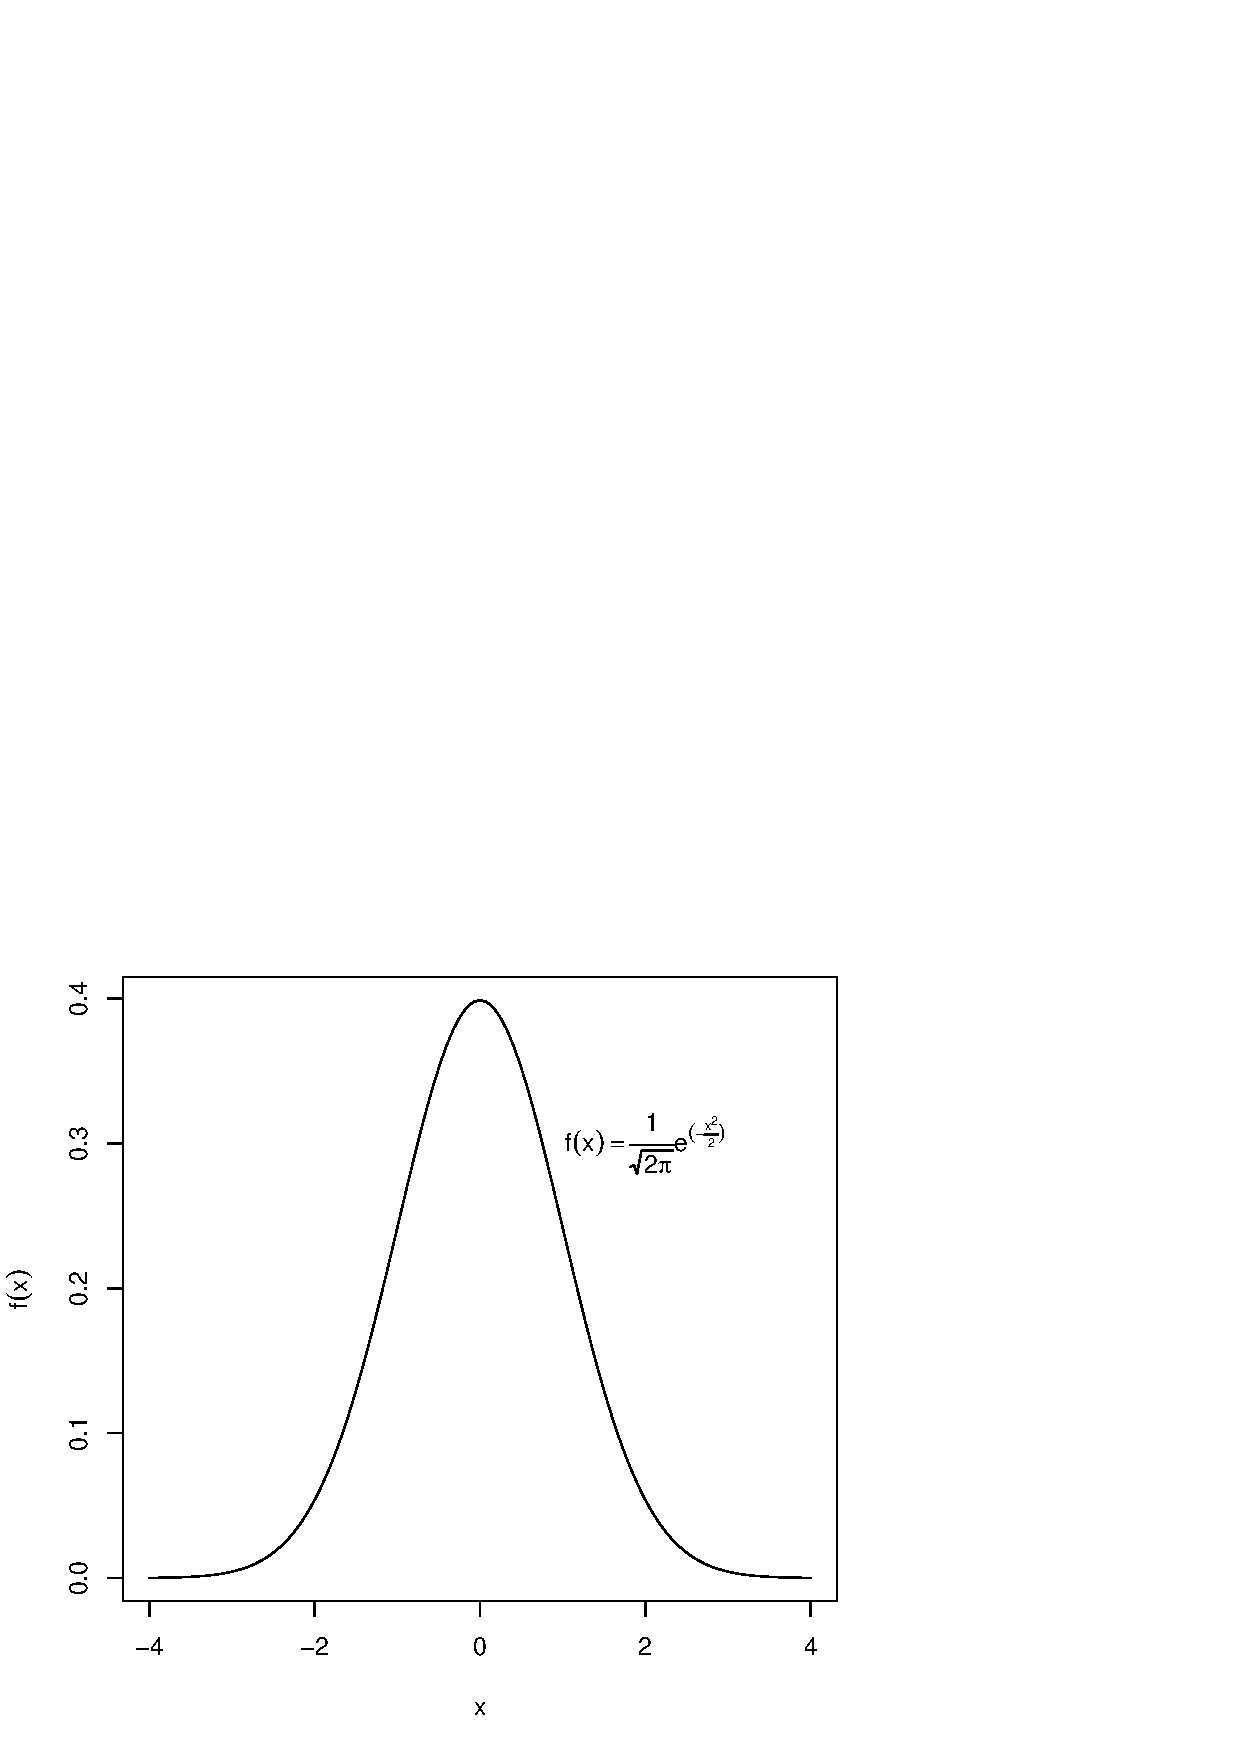
\includegraphics{./dibujos/02/-006}
\caption{Gráfica de la densidad gaussiana estándar}
\end{figure}
\end{center}
\end{frame}



\subsection{Variables absolutamente continuas}

\begin{frame}
\frametitle{Variables absolutamente continuas}
\begin{itemize}
\item Diremos que una v.a. tiene una ley \textbf{absolutamente continua} si su función de distribución se puede
escribir como 

$$\displaystyle F(x)=\int_{-\infty}^x f_{X}(t) dt$$ 

para todo $x\in\RR$.
\item  Donde $f$ es una función de densidad a la que llamaremos
función de densidad de la v.a. $X$
\item Cometeremos el abuso de decir \textbf{continua} una variable \textbf{absolutamente continua}.
\end{itemize}
\end{frame}

\begin{frame}
\frametitle{Propiedad}
Si $X$  es una v.a. tiene una función de distribución $F$ absolutamente continua se cumple que:
\begin{enumerate}[a)]
\item $F_{X}$ es continua.
\item Su funci\'on de densidad es $f(x)=F'_{X}(x)=\frac{d}{dx}F_{X}(x)$.
\item $D_X=\{x| f(x)>0\}$. Además $1=\int_{-\infty}^{\infty} f(x) dx=\int_{D_x} f(x) dx$.
\item Si  $A$ es un intervalo real, entonces $\displaystyle P(X\in A)=\int_{A} f(x) dx$.\newline
Por ejemplo si $A=(a,b]$ entonces 
$$\displaystyle P(X\in(a,b])=P(a<X\leq b)=\int_{a}^b f(x) dx.$$
\item Esta propiedad es similar para otro tipo de intervalos. 
\end{enumerate}
\end{frame}


\begin{frame}
\frametitle{Ejemplo}
\begin{itemize}
\item Supongamos que elegimos con ``equiprobabilidad'' un número al azar del intervalo real $(0,1)$.
\item Sea $X$ la v.a. que nos da ese número. 
\item Dado $0<x<1$ tenemos que 

$$P(X\leq x)=\frac{\mbox{longitud casos favorables}}{\mbox{longitud casos posibles}}= \frac{x-0}{1-0}=x.$$
\item Por lo tanto la función de distribución es 
$$F(x)=\left\{\begin{array}{ll} 0 &\mbox{ si } x\leq 0 \\
x  & \mbox{ si } 0<x<1\\
1 & \mbox{ si } x\geq 1
 \end{array}\right.
$$
\end{itemize}
\end{frame}

\begin{frame}
\begin{itemize}
\item La v.a. $X$  es absolutamente continua. Su función de densidad es 

$$
F'(x)=f(x)=\left\{\begin{array}{ll} 1 &\mbox{ si } 0 <x<1 \\
0 & \mbox{ en el resto de casos } 
 \end{array}\right.
$$

\item Ahora tenemos que  dado $0<x<1$

$$F(x)=\int_{-\infty}^x 1 dt =\int_{-\infty}^0 1 dt + \int_{0}^x t dt = \left.t\right|_{t=0}^{t=x}=x-0=x.$$
\item Efectivamente la integral de la función de densidad es la función de distribución.
\end{itemize}
\end{frame}

\begin{frame}
\frametitle{Ejemplo}

Sea $X$ una variable aleatoria con dominio $D_X=(1,2)$. Su función de densidad es:

$$f_X(x)=\left\{\begin{array}{ll}
k\cdot x^2+\frac{1}{3} & \mbox{ si } 0<x<1\\
0 & \mbox{en otro caso}
\end{array}\right.$$

Donde $k$ es una constante real ¿Cuál es el valor de $k$?

$1=\int_{0}^1 (k x^2+\frac{1}{3}) dx= \left.\left(k\frac{x^3}{3}+\frac{1}{3}x\right)\right|_{x=0}^{x=1}=
\left(k\frac{1}{3}+\frac{1}{3}\right)-(0+0)=\frac{k+1}{3}$

Resolviendo la ecuación  $1=\frac{k+1}{3}$ obtenemos que $k=2$.
\end{frame}

\begin{frame}
\frametitle{Gráfica de la función de densidad}
\begin{figure}
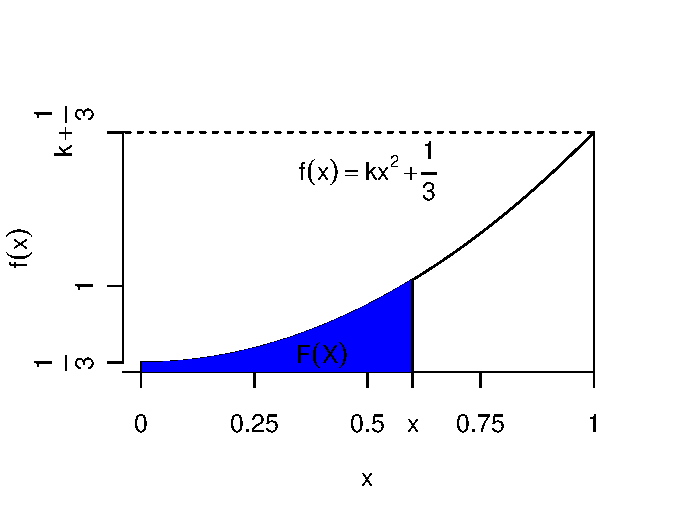
\includegraphics{./dibujos/02/-007}
\caption{Gráfica de una densidad y su  relación con la función de distribución.}
\end{figure}
\end{frame}

\begin{frame}
\begin{itemize}
\item En resumen,la función de densidad de la v.a. $X$ es 
$$f_X(x)=\left\{\begin{array}{ll}
2 x^2+\frac{1}{3} & \mbox{ si } 0<x<1\\
0 & \mbox{en otro caso}
\end{array}\right.$$
\item Dado $0<x<1$. la función de distribución es,

$F(x)=\int_{0}^x (2 t^2+\frac{1}{3}) dt =  \left.\left(2\frac{t^3}{3}+\frac{1}{3}t\right)\right|_{t=0}^{t=x}=
\left(2\frac{x^3}{3}+\frac{1}{3}x\right)=\frac{2 x^3+x}{3}.$
\end{itemize}
\end{frame}

\subsection{Esperanza y varianza para variables aleatorias continuas}

\begin{frame}
\frametitle{Esperanza de una variable aleatoria continua}
Sea $X$ una v.a. continua con función de densidad $f(x)$.
\begin{itemize}
\item Llamaremos \textbf{esperanza, media o valor esperado}  de la v.a. $X$ a 

           $$E(X)=\int_{-\infty}^{\infty}x \cdot f_{X}(x) dx$$
\item Si el  dominio de $X$ es  $D_X=(a,b)$ entonces

 $$E(X)=\int_{a}^{b}x \cdot f_{X}(x) dx$$ 
\end{itemize}
\end{frame}

\begin{frame}
\frametitle{Ejemplo}
Consideremos la v.a. $X$  con función de densidad:

$$
f(x)=\left\{\begin{array}{ll} 2 x^2+\frac{1}{3} &\mbox{ si } 0 <x<1 \\
0 & \mbox{ en el resto de casos } 
 \end{array}\right.
$$


Su valor esperado es 

\[
\begin{array}{rl}
E(X)= & \int_{0}^1 x \left(2 x^2 +\frac{1}{3}\right) dx= \int_{0}^1 \left(2 x^3 +\frac{1}{3}x\right) dx=
\left.\left(2 \frac{x^4}{4}+\frac{1}{3} \frac{x^2}{2}\right)\right|_{x=0}^{x=1} \\ = & \frac{1}{2}+\frac{1}{6}-(0+0)=\frac{2}{3}.
\end{array}
\]

\end{frame}




\begin{frame}
\frametitle{Esperanza de una función de una v.a.}
\begin{itemize}
\item  Sea $X$ una v.a. continua con densidad $f(x)$ y sea  $Y=g(X)$ una v.a. continua funci\'on de $X$. Entonces se define la \textbf{esperanza de la función} como :

$E(Y)=E(g(X))=\int_{-\infty}^{+\infty} g(x) f(x)dx$.
\item  Si el dominio de $X$ es $D_X=(a,b)$ entonces:
$E(Y)=E(g(X))=\int_{a}^{b} g(x) f(x)dx$.
\end{itemize}
\end{frame}


\begin{frame}
\frametitle{Ejemplo}
Consideremos la v.a. $X$  con función de densidad:

$$
f(x)=\left\{\begin{array}{ll} 2 x^2+\frac{1}{3} &\mbox{ si } 0 <x<1 \\
0 & \mbox{ en el resto de casos } 
 \end{array}\right.
$$


El valor esperado de la función $Y=X^2$ es:  

\[
\begin{array}{rl}
E(Y)= & E(X^2)=\int_{0}^1 x^2 \left(2 x^2 +\frac{1}{3}\right) dx= \int_{0}^1 \left(2 x^4 +\frac{1}{3}x^2\right) dx \\ = & 
\left.\left(2 \frac{x^5}{5}+\frac{1}{3} \frac{x^3}{3}\right)\right|_{x=0}^{x=1}=\frac{2}{5}+\frac{1}{9}-(0+0)=\frac{23}{45}.
\end{array}
\]

\end{frame}


\begin{frame}
\frametitle{Varianza de una v.a. continua}

Al igual que en el caso discreto, se define la \textbf{varianza} de una variable aleatoria continua como:

$$Var(X)=E(X-E(X)^2)$$

Se cumple que 

$$Var(X)=E(X^2)-E(X)^2$$

\end{frame}

\begin{frame}
\frametitle{Ejemplo}
Consideremos la v.a. $X$  con función de densidad:

$$
f(x)=\left\{\begin{array}{ll} 2 x^2+\frac{1}{3} &\mbox{ si } 0 <x<1 \\
0 & \mbox{ en el resto de casos } 
 \end{array}\right.
$$

Hemos visto anteriormente que $E(X)=\frac{2}{3}$ y $E(X^2)=\frac{23}{45}$. Por lo tanto su varianza es:

\[
Var(X)=E(X^2)-E(X)^2= \frac{23}{45}-\left(\frac{2}{3}\right)^2=\frac{1}{15}.
\]
\end{frame}


\begin{frame}
 \frametitle{Notaciones esperanzas y varianzas}
\begin{itemize}
\item De forma frecuente se denota por $\mu$ y $\sigma^2$ a la esperanza y varianza poblacionales de una distribución.
\item  La raíz cuadrada positiva de la varianza se denota por $\sigma$ y recibe el nombre de desviación típica poblacional.
\end{itemize}
\end{frame}

 \begin{frame}
\frametitle{Propiedades de la esperanza y la varianza}
\begin{enumerate}[a)]
\item $E(cte.)=cte$.
\item $E(a X+b)=a E(X)+b$.
\item $\displaystyle  E\left(\sum_{k=1}^{n }g_{k}(X)\right)=\sum_{k=1}^{n }E\left(g_{k}(X)\right)$.
\item Si $a<X<b$ entonces $a<E(X)<b$.
\item Si $X$ es una v.a. no negativa entonces $E(X)\geq 0$.
\item Si $g(X)\leq h(X)$ entonces $E(g(X))\leq E(h(X))$.
\item $Var(aX+b)=a^2 Var(X)$ donde $a,b$ son ctes. reales.
\item $Var(cte.)=0$
\end{enumerate}
\end{frame}

\section{Algunas modelos de distribuciones continuas}

\begin{frame}
\frametitle{Algunos  distribuciones continuas notables}
\begin{itemize}
\item En esta sección describiremos tres modelos de variables continuas.
\item Concretamente son: el modelo \textbf{uniforme}, el \textbf{exponencial} y el \textbf{gaussiano} o \textbf{normal}.
\item  A lo largo del curso, en la medida que sea necesario, expondremos otros modelos de distribuciones continuas como: la $t$ de \textbf{Student}, la \textbf{ji-cuadrado}, la $F$ de \textbf{Fisher}....
\item La función de distribución de estas distribuciones puede que no tenga una fórmula explícita.
\item En caso de no tener fórmulas explícitas se calcularan mediante tablas y usando \texttt{R}.
\end{itemize}
\end{frame}

\subsection{Distribución uniforme en el intervalo (a,b)}

\begin{frame}
\frametitle{Distribución uniforme}
 Una v.a. continua $X$ diremos que tiene una \textbf{distribución uniforme} sobre el intervalo real
$(a,b)$ ,$(a<b)$, si su función de densidad es
 $$f_X(x)=\left\{\begin{array}{ll}
\frac{1}{b-a} & \mbox{si } a<x<b\\ 0  & \mbox{en cualquier otro caso}
\end{array}
\right. $$ 
(como ejercicio comprobar que el área comprendida entre $f_X$ y el eje de abscisas (eje horizontal o eje~$X$)
vale~$1$.)

Si $X$ es una v.a. uniforme en el intervalo $(a,b),$ escribiremos $X\equiv U(a,b)$.

\end{frame}

\begin{frame}
Su función de distribución es:

$$F_X(x)=\left\{\begin{array}{ll} 0  & \mbox{si } x\leq a\\
\frac{x-a}{b-a} & \mbox{si } a<x<b\\ 1  & \mbox{si } b\leq x
\end{array}
\right. $$

Efectivamente:

\begin{itemize}
    \item Si $x\leq a$ entonces $F_X(x)=\int_{-\infty}^{x} f(t) dt= \int_{-\infty}^{x}
    0 dt =0$
    \item Si $a<x<b$ entonces $F_X(x)=\int_{-\infty}^{x} f(t) dt= \int_{-\infty}^{a}
    0 dt+\int_{a}^{x} \frac{1}{b-a} dt= 
    \frac{t}{b-a}\mid_{a}^{x}=\frac{x}{b-a}-\frac{a}{b-a}=\frac{x-a}{b-a}$
    \item  Por último si $x\geq b$ entonces $F_X(x)=\int_{-\infty}^{x} f(t)
    dt=1$ (ejercicio).
\end{itemize}
\end{frame}

\subsubsection{Esperanza y varianza  para $U(a,b)$}
\begin{frame}
\frametitle{Esperanza y varianza  para  una v.a. $X$ con distribución  $U(a,b)$}
\[
\begin{array}{rl}
E(X)= & \int_{-\infty}^{+\infty} x f_X(x) dx=\int_{a}^{b} x \frac{1}{b-a} dx =
\frac{x^2}{2(b-a)}\mid _{a}^{b}=\frac{b+a}{2}, \\ & \\
E(X^2)= & \int_{-\infty}^{+\infty} x^2 f_X(x) dx=\int_{a}^{b} x^2 \frac{1}{b-a}
dx =\frac{x^3}{3(b-a)}\mid_{a}^{b} =\frac{b^3-a^3}{3(b-a)} \\ = & \frac{b^2+ab+a^2}{3}, \\ & \\
Var(X)= & E(X^2)-(E(X))^2=\frac{b^2+ab+a^2}{3}-(\frac{b+a}{2})^2=\frac{(b-a)^2}{12}.
\end{array}
\]
\end{frame}

\begin{frame}
\frametitle{Gráfica de la distribución $U(-1,2)$}
\begin{figure}[h]
\begin{center}
\scalebox{0.6}[0.6]{
\begin{tabular}{cc}       
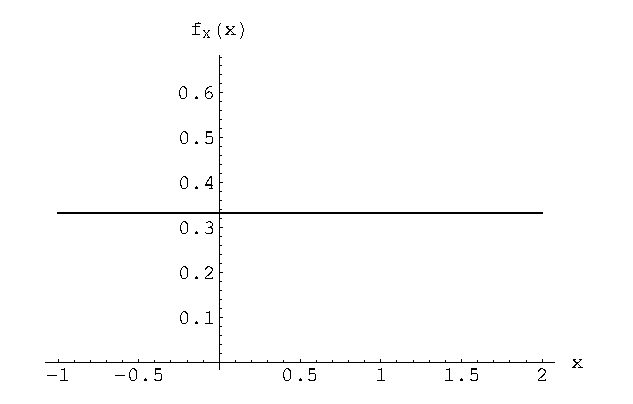
\includegraphics[scale=0.5]{densidaduniforme12}
&
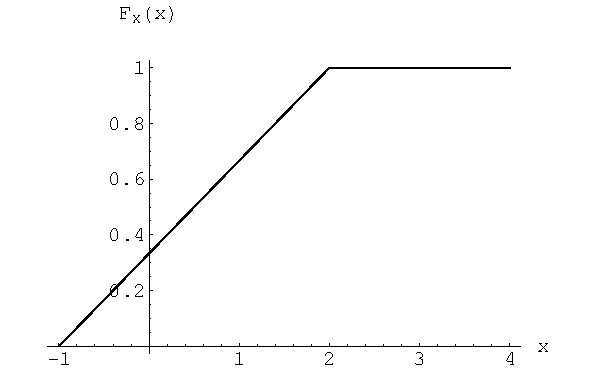
\includegraphics[scale=0.5]{distribucionuniforme12}\\
 a) & b) 
\end{tabular}
}
\end{center}
\caption{ Gráficas de la función de densidad (a)  y de la función de distribución (b) de una v.a. $U(-1,2)$.}
\end{figure}
\end{frame}

\subsubsection{Resumen v.a con distribución uniforme, $U(a,b)$}

\begin{frame}
\scalebox{0.8}[0.8]{
\begin{tabular}{|c|c|c|c|c|}
\hline \begin{tabular}{c} Valores\\ admisibles.\end{tabular} & $f_{X}(x)$ & $F_X(x)=P(X\leq
X)=$ &
 $E(X)$ & $Var(X)$\\\hline & & & &\\
 $D_X=(a,b)$ & $\left\{\begin{array}{ll}
\frac{1}{b-a} & \mbox{si } a<x<b\\ 0  & \mbox{en cualquier otro caso}
\end{array}
\right.$  &  $\left\{\begin{array}{ll} 0 & \mbox{ si } x\leq a\\
          \frac{x-a}{b-a} & \mbox{ si } a\leq x\leq\\
          1 & \mbox{ si } b\leq x\end{array}\right.$
 & $\frac{a+b}{2}$ & $\frac{(b-a)^2}{12}$ \\& & & &\\ \hline
\end{tabular}
}
\end{frame}
\subsection{Distribución exponencial (exponencial negativa)}
\begin{frame}

\frametitle{Modelo exponencial}

\begin{itemize}
\item      Supongamos que tenemos un proceso Poisson con parámetro $\lambda$ en una unidad de tiempo.
\item    Entonces dadas $t$ unidades de tiempo tenemos que $X_{t}=$ número de eventos en el intervalo de tiempo $(0,t]$ es una $Po(\lambda\cdot t)$. 
\item Consideremos la v.a. $T=$tiempo transcurrido entre dos eventos Poisson consecutivos.
\item Dado $t>0$, tenemos que 
$P(T>t)=P(\mbox{Cero eventos en el intervalo}(0,t])=P(X_{t}=0)= $
$\frac{(\lambda t)^0}{0!} e^{-\lambda t}=e^{-\lambda t}.$
\end{itemize}
\end{frame}

\begin{frame}
\begin{itemize}
\item   Tomando complementarios, la función de distribución de $T$ será

         $$F_{T}(t)=P(T\leq t)=\left\{\begin{array}{ll} 0 &\mbox{ si } t\leq 0\\
          1-P(T>t)=1-e^{-\lambda t}& \mbox{ si } t>0\end{array}\right.$$
\item Por lo tanto
         $$f_{T}(t)=\left\{\begin{array}{ll}
         \lambda e^{-\lambda t} & \mbox{ si }  t>0\\
         0 & \mbox{ si } t\leq 0
         \end{array}\right.$$
\item Ésta es la distribución exponencial y la denotaremos por $Exp(\lambda)$
\end{itemize}
\end{frame}

\begin{frame}
\frametitle{Propiedad de la falta de memoria}
Sea $X$  una v.a. $Exp(\lambda)$ entonces

          $$P(X>s+t/X>s)=P(X>t)\mbox{  para todo } s,t\in \RR$$

          Toda v.a. absolutamente continua, que tome valores positivos
          y que verifique la propiedad de la falta de memoria es una v.a.
          exponencial.
\end{frame}


\subsubsection{Resumen v.a con distribución exponencial, $Exp(\lambda)$}

\begin{frame}

Sea $X\equiv Exp(\lambda).$

%\begin{center}ç
\scalebox{0.7}[0.7]{
\begin{tabular}{|c|c|c|c|c|}
\hline \begin{tabular}{c} Valores\\ admisibles.\end{tabular} & $f_{X}(x)$ & $F_X(x)=P(X\leq
X)=$ &
 $E(X)$ & $Var(X)$\\\hline & & & &\\
 $D_X=(0,+\infty)$ & $\left\{\begin{array}{ll}
         \lambda e^{-\lambda x} & \mbox{ si }  x>0\\
         0 & \mbox{ si } x\leq 0
         \end{array}\right.$ &  $F_{X}(x)=P(X\leq x)=\left\{\begin{array}{ll} 0 &\mbox{si } x\leq 0\\
          1-e^{-\lambda x}& \mbox{si } x>0\end{array}\right.
$ & $\frac{1}{\lambda}$ & $\frac{1}{\lambda^2}$ \\& & & &\\ \hline
\end{tabular}
%\end{center}
}
\end{frame}
%\end{document}
\subsection{Distibución normal o gaussiana}

\begin{frame}
\frametitle{Distribución normal o Gaussiana}
Diremos que una v.a. $X$ sigue una \textbf{ley normal} o \textbf{gaussiana} de parámetros $\mu$ y $\sigma$ y lo denotaremos por $N(\mu,\sigma)$ si tiene por funci\'on de densidad:

$$f_{X}(x)=\frac{1}{\sqrt{2\pi}\sigma} e^{\frac{-(x-\mu)^2}{2\sigma^{2}}} \mbox{ para todo } x\in \RR$$

La gráfica de esta función es la conocida campana de Gauss, que ya hemos dibujado dos veces.  La v.a. normal con $\mu=0$ y $\sigma=1$ recibe el
nombre de normal est\'andard. 

La normal estándard se suele denotar por la letra $Z$ y su función de distribución $F_Z$.
\end{frame}

\begin{frame}
\frametitle{Propiedades} 
Sea $X$ una v.a. $N(\mu,\sigma^2)$ y sea $f_{X}$ su funci\'on de densidad. Entonces:
\begin{enumerate}[a)]
\item Evidentemente $f_{X}$ verifica todas las propiedades de las funciones de densidad.
\item $f_{X}(\mu-x)=f_{X}(\mu+x)$ es simétrica respecto de la recta $x=\mu$
\item $f_{X}$ alcanza el máximo en $x=\mu$
\item Si $F_{X}$ la función de distribución de $X$ entonces  $F_{X}(\mu+x)=1-F_{X}(\mu-x)$. En particular si $Z$ es una $N(0,1)$ entonces $F_{Z}(-x)=1-F_{Z}(x)$
\item $Z=\frac{X-\mu}{\sigma}$ es una v.a. $N(0,1)$ y $X=\sigma Z+\mu$ es una $N(\mu,\sigma^{2})$ donde $Z$ es la normal estándar.
\end{enumerate}
\end{frame}


%%%%%aqui
\begin{frame}
\frametitle{Importancia  y propiedades de la distribución normal}
\begin{itemize}
\item  La variable aleatoria normal es una de las más importantes de la estadística.
\item  La justificación es que la distribución de muchos estadísticos como la media o la proporción muestral se aproximan  a una distribución normal cuando los tamaños de las muestras son grandes.
\item 
Como ya hemos visto en distribuciones continuas las probabilidades se calculan como áreas que se forman debajo de una curva, llamada curva de densidad, y el eje horizontal.
 \item  Como en todas las distribuciones continuas la probabilidad $P(X\leq x)$. es el área comprendida entre el eje horizontal la curva normal y la vertical que corta al eje horizontal en $x$, ver la fig.~\ref{areacurvanormalgeneralderecha}.
\end{itemize}
\end{frame}
 
\begin{frame}[fragile]
\begin{figure}[htbp]
\begin{center}
%\includegraphics{areacurvanormalgeneralderecha.eps}
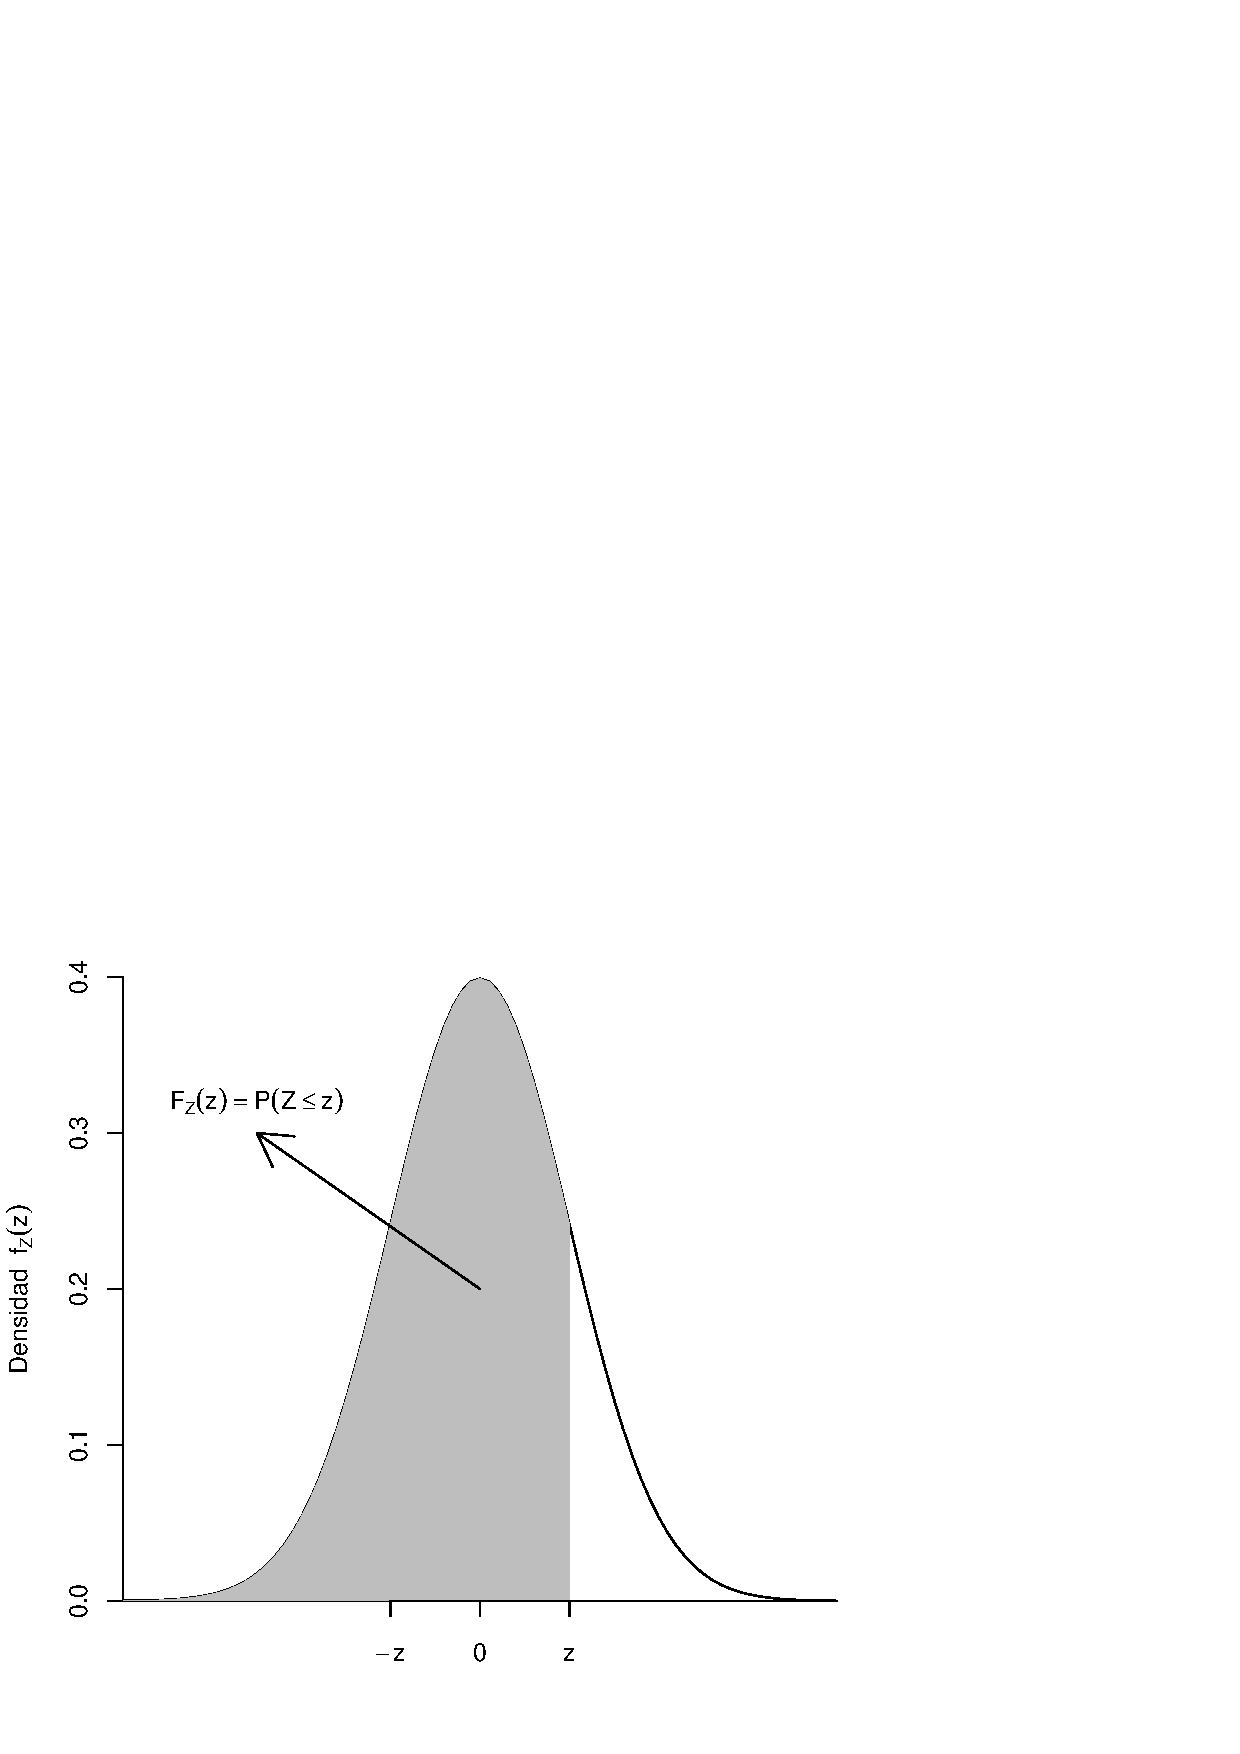
\includegraphics{./dibujos/02/-008}

\end{center}
\caption{la $P(X\leq x)$ como un área bajo la curva normal.}
	\label{areacurvanormalgeneralderecha}
\end{figure}
\end{frame}
 
 \subsubsection{Comportamiento de la curva normal}
\begin{frame}
\begin{itemize}
\item  La curva normal toma distintas formas en función del valor de sus pa\-rá\-me\-tros.
\item  Consideremos dos curvas normales con medias $\mu_1=\mu_2$ respectivamente y varianzas $\sigma_1^2<\sigma_2^2$.
\item  Las dos curvas estarán centradas en la media, pero la segunda será más achatada, pues tiene varianza mayor y los valores se alejan más  del valor medio.
\item  Este caso se ilustra en la fig.~\ref{dosnormalesmediasigualesvardistintas}
 \end{itemize}
\end{frame}

\begin{frame}
 
 \begin{center}
\begin{figure}[htbp]
	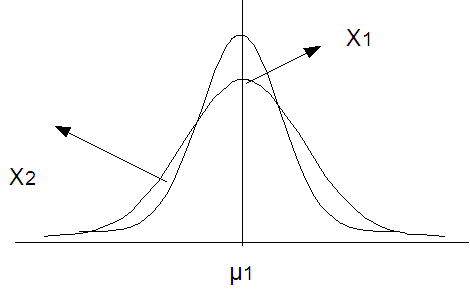
\includegraphics{dosnormalesmediasigualesvardistintas.png}
	\caption{Dos curvas normales $X_1$ y $X_2$ con $\mu_1=\mu_2$ y $\sigma_1^2<\sigma_2^2$.}
	\label{dosnormalesmediasigualesvardistintas}
\end{figure}
\end{center}
\end{frame}

\begin{frame}

En el caso en que las varianzas sean iguales y las medias distintas, las curvas normales tienen la misma forma pero cada una de ellas está centrada en cada una de sus medias. El efecto puede verse en la fig.~\ref{dosnormalesmediasdistintasvariguales}



\begin{center}
\begin{figure}[htbp]
	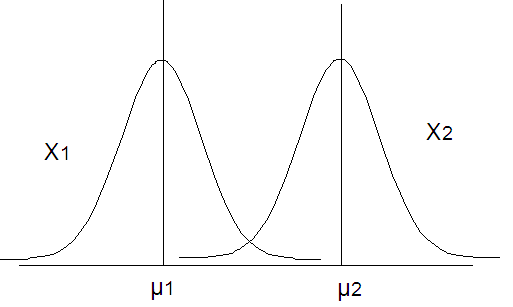
\includegraphics{dosnormalesmediasdistintasvariguales.png}
	\caption{Dos curvas normales $X_1$ y $X_2$ con $\mu_1<\mu_2$ y $\sigma_1^2=\sigma_2^2$.}
	\label{dosnormalesmediasdistintasvariguales}
\end{figure}
\end{center}
\end{frame}
\begin{frame}
Por último si las medias son distintas y las varianza también se obtienen curvas como las de la fig.~\ref{dosnormalesmediasdistintasvardistintas}

 \begin{center}
\begin{figure}[htbp]
	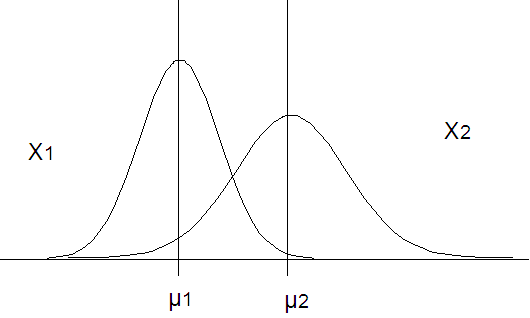
\includegraphics[scale=0.8]{dosnormalesmediasdistintasvardistintas.png}
	\caption{Dos curvas normales $X_1$ y $X_2$ con $\mu_1<\mu_2$ y $\sigma_1^2<\sigma_2^2$.}
	\label{dosnormalesmediasdistintasvardistintas}
\end{figure}
\end{center}
\end{frame}




\subsubsection{Estandarización de la variable normal}
\begin{frame}
\frametitle{Estandarización de la variable normal}

\begin{itemize}
\item La estandarización o tipificación de una variable ya fue comentada en el primer tema.
\item  Consiste en transformar una variable o una serie de datos a unos datos típicos o estándars en el sentido que todos tengan esperanza o media $0$ y varianza poblacional o muestral igual a $1$. 
\item Para conseguir este efecto es suficiente restar a la variable la media y dividir el resultado por la desviación típica. Estas ideas ya se vieron en el módulo anterior.
\end{itemize}

\end{frame}
\begin{frame}
\begin{itemize}
\item En general supongamos que tenemos un variable $X$ con valor esperado $\mu$ y desviación típica $\sigma$. Entonces sus puntuaciónes estándar (\textit{$z$-scores}) se suele denotar por la letra $Z$ se calculan como $Z=\frac{X-\mu}{\sigma}$.
para la versión  poblacional
\item Mientras que para la versión muestral, como ya vimos, es $=\frac{x-\overline{x}}{s}$
\end{itemize}
\end{frame}

\begin{frame}
\begin{itemize}
\item La variable o serie de datos $Z$ tiene esperanza o media $0$ y varianza poblacional o muestral $1$. 
\item En este sentido es una variable de puntuaciones estándar y puede servirnos para comparar las puntuaciones de dos variables o series de datos
\item  Este es el motivo por el que recibe el nombre de estándar, pues reduce los datos o variables a ``\textsl{unidades estándar}". \item Existen otras  formas de reducir variables o series a puntuaciones que sean comparables. 
\end{itemize}
\end{frame}

\subsubsection{Estandarización de la variable normal}
\begin{frame}
\begin{itemize}
\item Para el caso de la variable aleatoria normal tenemos una propiedad importante. 
\item Es suficiente conocer todas las probabilidades de una variable aleatoria $Z$ normal estándar o típica es decir con $\mu=0$ y $\sigma=1$ para conocer las probabilidades de cualquier variable normal de media $\mu$ y desviación típica $\sigma$.
\item  La igualdad que relaciona estas dos probabilidades es
$$P(X\leq x)=P(Z\leq \frac{x-\mu}{\sigma}).$$
Donde $Z$ es una variable que sigue la ley normal estándar, es decir una normal con $\mu=0$ y $\sigma=1$.
\item Lo que nos dice esta propiedad es que cuando $X$ es una variable aleatoria con distribución normal de parámetros $\mu$ y $\sigma^2$, la variable $Z=\frac{X-\mu}{\sigma}$ sigue una distribución normal estándar.
\item A la función que nos da las probabilidades de la variable normal estándar $Z$  la denotaremos por $F_Z(z)=P(Z\leq z).$
\end{itemize}
\end{frame}

\begin{frame}

Es sencillo comprender mirando la fig.~\ref{areanormalestandarderecha} que la función de distribución de la variable normal estándar cumple la propiedad: $F_Z(-z)=1-F_Z(z).$

 \begin{center}
\begin{figure}[htbp]
	%\includegraphics[scale=0.8]{areanormalestandarderecha.pdf}
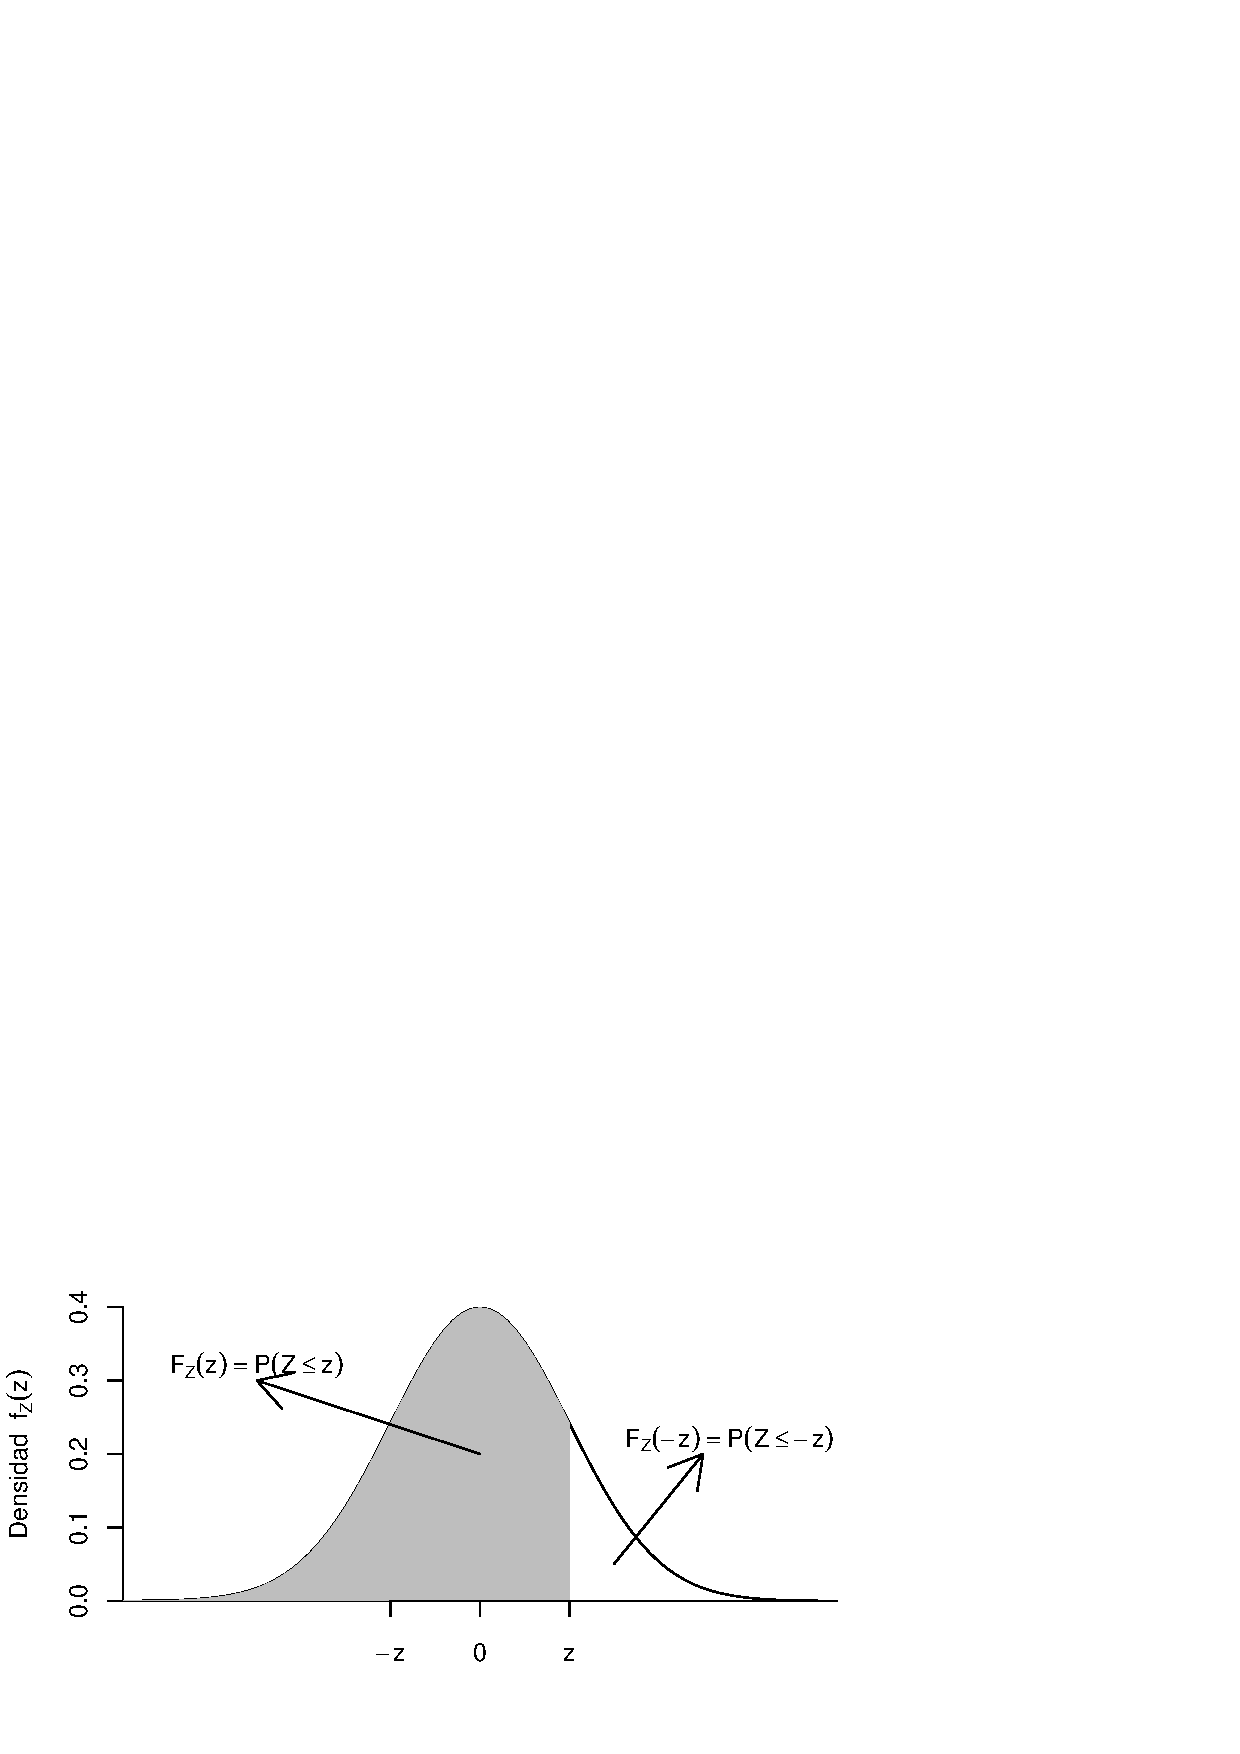
\includegraphics{./dibujos/02/-009}

\caption{Justificación gráfica de la propiedad de la normal estándar: $F_Z(-z)=1-F_Z(z)$.}
	\label{areanormalestandarderecha}
\end{figure}
\end{center}

\end{frame}


\begin{frame}

\subsubsection{Uso de tablas para el cálculo de la función de distribución normal.}
\begin{itemize}
\item Las  tablas para el cáculo de la normal están disponibles  en ``http://bioinfo.uib.es/\~{}recerca/mates2/tablasDistribuciones/''.
\item Estas tablas contienen los valores de la distribución normal estándar. Es decir los valores de  $F_{Z}(z)=P(Z\leq z)$ para una variable
$Z$ normal estándar.
\item  La primera tabula los valores negativos y la segunda, los positivos. Por ejemplo $F_{Z}(1.78)=0.9625$, es un resultado que se encuentra en la
segunda tabla. Si queremos saber el valor de $F_Z(-1.78)=1-F_Z(1.78)=0.0375$ donde hemos utilizado la propiedad $F_Z(-z)=1-F_Z(z)$.
\item La entrada horizontal de la tabla es el segundo decimal del número que buscamos, mientras que la primera columna contiene las unidades y el
primer decimal.
\item Si queremos calcular la probabilidad de que $Z$ esté comprendida entre $-2$ y $2$ 
\item $P(-2\leq Z\leq 2)=F_Z(2)-F_Z(-2)=0.9772-0.0228=0.9544.$
\end{itemize}
\end{frame}

\begin{frame}
\begin{itemize}
\item La explicación es la siguiente: la probabilidad de que $Z$ esté entre $-2$ y $2$ es el área comprendida bajo la curva normal, el eje horizontal
y las verticales que pasa por $-2$ y $2$.
\item  Este área es el área encerrada bajo la curva y  menor o igual que~$2$ menos el área encerrada bajo la curva y menor que~$-2$.
\item En general se tiene que 
$P(a\leq Z\leq b)=P(Z\leq a)-P(Z\leq b)=F_Z(a)-F_Z(b).$
\item En particular dado $\delta>0$ entonces
$P(-\delta\leq Z \leq \delta)=F_{Z}(\delta)-F_{Z}(-\delta).$
\item \textbf{Nota:} En el caso de variables continua los $\leq$ se pueden cambiar por $<$ (uno todos o ninguno) y las probabilidades no varían. Es decir $P(Z\leq a)=P(Z< a)$.
\end{itemize}
\end{frame}

\begin{frame}

\frametitle{Ejemplo} 
Sea $Z$ una variable normal estándar. Utilizando las tablas de la distribución normal estándar calcular las siguientes probabilidades:
\begin{enumerate}[a)]
\item $P(0< Z < 3.99)=F_Z(3.99)-F_Z(0)\approx 1-0.5=0.5$. 
\item $P(-3.99\leq Z \leq 3.99)=F_{Z}(3.99)-F_{Z}(-3.99)\approx 1.$
\item $P(-3\leq Z \leq 3)=F_{Z}(3)-F_{Z}(-3)= 0.9987-0.0013=0.9974$.
\item $P(Z\leq -2)=F_Z(-2)=0.0228$.
\item $P( Z \leq 2)=F_{Z}(2)=0.9772$.
\item $P( Z \geq 2)=1-P(Z<2)=1-F_{Z}(2)=0.0228$.
\item $P( Z \geq -2)=1-P(Z< -2)=1-F_{Z}(-2)=1-(1-F_Z(2))=F_Z(2)$.
\item Dado $\delta>0$, $P(-\delta\leq Z \leq
\delta)=F_{Z}(\delta)-F_{Z}(-\delta)=F_Z(\delta)-(1-F_Z(\delta))=2\cdot  F_Z(\delta)-1$.
\item Utilizando la igualdad anterior
$P(-2\leq Z \leq 2)=2\cdot  F_Z(2)-1=2 \cdot 0.9772-1=0.9544$.
\end{enumerate}

\end{frame}


\begin{frame}

\begin{itemize}
\item No sólo podemos utilizar la tabla para calcular la probabilidad en un valor determinado. 
\item También la podemos utilizar para calcular los cuantiles de $Z$ que tienen la misma definición que vimos en estadística descriptiva.
\item  Por ejemplo si quiero calcular el valor $z$ tal que $P(Z\leq z)=0.9099$ buscamos dentro de la tabla el valor $0.9099$, o el más cercano, en este caso es $F_Z(1.34)=0.9099$ por lo tanto el valor buscado es $z=1.34$.
\end{itemize}
\end{frame}

\begin{frame}

\frametitle{Ejemplo}
 Calcular los valores que se piden para una variable $Z$ normal estándar.
\begin{enumerate}[a)]
\item Calcular el valor $z$ tal que $P(Z\leq z)=0.504$. Mirando las tablas se obtiene que  $F_Z(0.01)=0.504$ por lo tanto el valor pedido es $z=0.01$.
\item Calcular el valor $z$ tal que $P(Z> z)=0.9633$. Primero hacemos el complementario $P(Z>z)=1-P(Z<z)=1-F_Z(z)=0.9633$. Ahora despejando obtenemos que  el valor buscado cumple
que $F_Z(z)=1-0.9633= 0.0367$. Mirando dentro de las tablas se obtiene que $F_Z(-1.79)=0.0367$. En definitiva el valor buscado es $z=-1.79$
\end{enumerate}
\end{frame}



\begin{frame}
\frametitle{Cáculo de probabilidad de una v.a. $N(\mu,\sigma)$.}
\begin{itemize}
\item Sólo nos queda ver como calculamos las probabilidades de una variable aleatoria normal de media $\mu$ y varianza $\sigma^2$.
\item  Recordemos la relación básica que dice que la variable tipificada de una normal sigue una ley normal estándar. Si $X$ es una normal de media
$\mu=1$ y varianza $\sigma^2=4$ se tiene que 
$$Z=\frac{X-\mu}{\sigma}=\frac{X-1}{2}$$

sigue una ley  normal estándar.
\item Por lo tanto   $P(X\leq x)=F_Z(\frac{x-\mu}{\sigma})$.
\end{itemize}
\end{frame}

\begin{frame}
\frametitle{Ejemplo}
\begin{enumerate}[a)]
\item 
Por ejemplo $P(X\leq 2)=P(\frac{X-1}{2}\leq \frac{2-1}{2})=P(Z\leq \frac{1} {2})=F_Z(0.5)=0.6915$.
\item Si queremos calcular el cuantil $0.6915$ de la variable $X$ será aquel valor $X$ tal que $P(X\leq x)=0.6915$. Tipificamos la variable $X$

$$P(X\leq x)=P(\frac{X-1}{2}\leq \frac{x-1}{2})=P(Z\leq \frac{x-1} {2})=F_Z(\frac{x-1} {2})=0.6915 ,$$

mirando en las tabla de la normal estándar resulta que $F_Z(0.5)=0.6915$, entonces 

$$ \frac{x-1} {2}=0.5 ,$$

despejando $x$ de la ecuación anterior se obtiene que $x=2\cdot 0.5+1= 2$.
\end{enumerate}
\end{frame}
 
 
 
 \begin{frame}
\frametitle{Resumen propiedades de la normal}
Resumiendo podemos utilizar las siguientes propiedades, $X\equiv N(\mu,\sigma)$
    \begin{itemize}
    \item  $Z$ es su variable tipificada, es decir,
    $Z=\frac{X-\mu}{\sigma}\equiv N(0,1)$ entonces:

    $$P(X\leq x)=P(\frac{X-\mu}{\sigma}\leq
    \frac{x-\mu}{\sigma})=F_{Z}(\frac{x-\mu}{\sigma})$$

   \item  Cuando tengamos un intervalo
    $$P(a<X<b)=P(\frac{a-\mu}{\sigma}<\frac{X-\mu}{\sigma}<\frac{b-\mu}{\sigma})=$$

    $$=P(\frac{a-\mu}{\sigma}<Z<\frac{b-\mu}{\sigma})=F_{Z}(\frac{b-\mu}{\sigma})-
    F_{Z}(\frac{a-\mu}{\sigma})$$
    \item Si $\delta>0$ $P(\mu-\delta\leq X \leq
\mu+\delta)=2 F_Z(\frac{\delta}{\sigma})-1$
\end{itemize}
\end{frame}

\begin{frame}
\frametitle{Ejemplo}
Sea $X$ una normal com media $2$ y varianza $4$, entonces
    \begin{enumerate}[a)]
\item  $P(1< X< 2)= P(\frac{1-2}{2}<\frac{X-2}{2}<\frac{2-2}{2})=
    P(\frac{-1}{2}<Z<0)=F_{Z}(0)-F_{Z}(-0.5)=\frac{1}{2}-1+F_{Z}(0.5).$
    \item $P(X>3)=P(\frac{X-2}{2}>\frac{3-2}{2})=
    P(Z>0.5)=1-F_{Z}(0.5).$
    \end{enumerate}
\end{frame}


\begin{frame}
\frametitle{Aproximación de una Binomial por una distribución normal}
\begin{itemize}
\item  Bajo determinadas condiciones la distribución normal puede aproximar a la distribución binomial.
\item  Sea $X$ una v.a. con distribución $B(n,p)$ entonces $E(X)=np$  y $Var(X)=npq$.
\item Sea $Z=\frac{X-E(X)}{\sqrt{Var(X)}}=\frac{X-np}{\sqrt{np(1-p)}}$.
\item Si $n$ es grande y $p$ no está muy cercano a $0$ o a $1$ la distribución de $Z$ se aproxima a una normal estándar.
\item La aproximación se realiza de la siguiente manera
$P(X=k)\approx P\left({{k-0.5-np}\over \sqrt{npq}}\leq Z \leq {{k+0.5-np}\over
\sqrt{npq}}\right)$
\item Mediante un razonamiento similar : $$\ P(X\leq k)\approx P\left(Z \leq
{{k+0.5-np}\over \sqrt{npq}}\right)$$
\item Y también $\ P(a\leq X\leq b)\approx\approx P\left(\frac{a-0.5-np}{\sqrt{npq}}\leq Z \leq \frac{b+0.5-np}{\sqrt{npq}}\right)$
\item Donde, en todos los  casos $Z$ se toma como una normal estándar.
\end{itemize}
\end{frame}
%%%%%%s%%
%%%%%%%%\textbf{Criterio:} La aproximaci�n es fiables si $np(1-p)>9$ y $n\geq 20$ y $p$ pr�ximo a
%%%%%%%%0.5
\begin{frame}
\frametitle{Corrección de continuidad} 
\begin{itemize}
\item El motivo de sumar o restar 0.5 en las aproximaciones es
corregir el efecto que tienen aproximar una v.a. discreta por una continua.
\item Esta operación recibe el nombre de corrección de continuidad de Fisher. 
\item Gráficamente el área que hacemos
corresponder a la probabilidad de cada valor entero $k$ en una binomial corresponde a la
comprendida entre la curva normal y el  segmento centrado en $k$ de amplitud 1.
\end{itemize}
\end{frame}

\begin{frame}
\frametitle{Ejemplo}
    $X$=número de caras en 100 lanzamientos de una moneda.
    $P(\mbox{cara})=\frac{1}{2}$. Calcular:

    \begin{enumerate}[a)]
    \item $P(40\leq X\leq 49)$
    \item $P(X=37)$
    \item $P(X\leq 50)$
    \end{enumerate}
    Solución:

    $E(X)=50=\mu_{X}$, $Var(X)=25$ y $\sigma_{X}=5$

    $Z=\frac{X-50}{5}$   se  aproxima a  normal  estándar
    %%%%%%%%y tenemos que
%%%%%%%%    $n=1000$, $np(1-p)=25$ y $p=0.5$

    Entonces....

\end{frame}

\begin{frame}
\begin{enumerate}[a)]
\item     
\[
\begin{array}{rl}
P(40\leq X\leq 49)\approx & P(\frac{40-0.5-50}{5}\leq Z\leq
    \frac{49+0.5-50}{5}) \\ = & P(-\frac{10.5}{5}\leq Z\leq -\frac{0.5}{5})=
    F_{Z}(-\frac{0.5}{5})-  F_{Z}(-\frac{10.5}{5}) \\ = & 
    1-F_{Z}(\frac{0.5}{5})-1+F_{Z}(\frac{10.5}{5})=
F_{Z}(\frac{10.5}{5})-F_{Z}(\frac{0.5}{5}) \\ = & F_{Z}(2.1)-F_{Z}(0.1)=0.9821-0.5398=0.4423.
\end{array}
\]

La probabilidad exacta da $0.442605$. ¡¡La aproximación es bastante buena!!

\item 
\[
\begin{array}{rl}
P(X=37)= & P(37\leq X\leq 37)\approx P(\frac{37-0.5-50}{5}\leq Z\leq
\frac{37+0.5-50}{5}) \\  = & P(-\frac{13.5}{5}\leq Z\leq -\frac{12.5}{5})=
F_{Z}(\frac{13.5}{5})+F_{Z}(\frac{12.5}{5}) \\  = & F_{Z}(2.7)-F_{Z}(2.5)= 0.9965-0.9938=0.0027.
\end{array}
\]

La probabilidad exacta da $0.0026979$. ¡¡La aproximación es bastante buena!!


\item $P(X\leq 50)\approx P(Z\leq \frac{50+0.5-50}{5})=P(Z\leq 0.5)=F_{Z}(0.1)=0.5398$

La probabilidad exacta calculada con un programa adecuado  da $0.539795$ ¡¡La aproximación
es bastante buena!!
\end{enumerate}
\end{frame}

\begin{frame}

\frametitle{Aproximación de una Poisson por una distribución normal}
\begin{itemize}
\item De forma similar a la aproximación de una binomial por una normal podemos aproximar la
probabilidad de una v.a. Poisson por una normal.
\item  Tendremos que aplicar también la corrección de continuidad.
\item Si $X\equiv Po(\lambda)$ y $\lambda$ es grande, entonces podemos usar
estas aproximaciónes:
\begin{itemize}
\item $ P(X=k) \approx P\left({{k-0.5-\lambda} \over
\sqrt{\lambda}}\leq Z \leq {{k+0.5-\lambda}\over \sqrt{\lambda}}\right)$
\item $P(X\leq k)\approx P\left(Z \leq
{{k+0.5-\lambda}\over \sqrt{\lambda}}\right)$
\item $P(a\leq X\leq b)\approx P\left(\frac{a-0.5-\lambda}{
\sqrt{\lambda}}\leq Z \leq \frac{b+0.5-\lambda}{ \sqrt{\lambda}}\right)$
\end{itemize}
\end{itemize}
\end{frame}

\begin{frame}
    \frametitle{Ejemplo}
    Sea $X$=número de trabajos que llegan a un centro de cálculo en
    un lapso de $60$ minutos.

    Supongamos que $X$ sigue una ley Poisson y que el número medio de
    trabajos que llegan por minuto sea $0.2$.
    Entonces $E(X)=0.2\cdot60=12$ por lo tanto $X$ es una $Po(12)$ es
    decir $\lambda =12$ y por lo tanto $\mu_X=12$ y $\sigma_X^2=12$.

    Si queremos calcular

    $P(Y\leq 10)\approx P(Z\leq \frac{10+0.5-12}{\sqrt{12}})=P(Z\leq -0.4330127)$

  $F_{Z}(-0.4330127)\approx 1-F_{Z}(0.43)=1-0.6664=0.3336$

La probabilidad exacta\footnote{Con R es  ppois(10,12) }  da $0.347229$. La aproximación es  buena.
\end{frame}

\begin{frame}
\frametitle{Conclusión}
\begin{itemize}
\item Si $X$ es una $B(n,p)$ entonces $E(X)=np$ y $Var(X)=npq$
\item Si $X$ es una $Po(\lambda)$ entonces $E(X)=Var(X)=\lambda$
\item Si $X$ es una $Ge(p)$ con $X(\Omega)=\{1,2,3,\ldots\}$  entonces $E(X)=\frac{1}{p}$ y $Var(X)=\frac{q}{p^2}$
\item Si $X$ es una $Ge(p)$ con $X(\Omega)=\{0,1,2,3,\ldots\}$ entonces $E(X)=\frac{q}{p}$ y $Var(X)=\frac{q}{p^2}$
\item Si $X$ es una $U(a,b)$ entonces $E(X)=\frac{a+b}{2}$ y $Var(X)=\frac{(b-a)^2}{12}$
\item Si $X$ es una $Exp(\lambda)$ $E(X)=\frac{1}{\lambda}$ y $Var(X)=\frac{1}{\lambda^2}$
\item Si $X$ es una $N(\mu,\sigma^2)$ $E(X)=\mu$ y $Var(X)=\sigma^2$
\end{itemize}
\end{frame}

